\section{Duality in consumer and producer theory}\label{sec:B-duality}

Duality theory studies an optimization problem through its value function. Under convexity the value
function summarizes the problem completely, and its derivatives deliver the demand or supply functions. The
envelope theorem of \cref{sec:B-envelope} computes those derivatives, so this section applies it repeatedly.
Empirical IO uses this in three ways. It builds demand systems from an expenditure function, as in the
almost ideal demand system of \cref{ch:aids}. It measures welfare exactly from estimated demand, as in the
valuation of new goods in \cref{ch:newgoods}. It recovers marginal cost from a cost function, as in the
conduct and airline studies of \cref{ch:conduct} and \cref{ch:airlines}. \Cref{sec:05-duality} proves the
consumer-theory results that the AIDS needs. This section restates them for reference and points to those
proofs. It adds five tools: the envelope-theorem proof of Shephard's lemma, the properties of indirect
utility, the integrability method of \citet{Hausman1981}, quasi-linear utility and producer duality.

There are $n$ goods indexed by $i, j = 1, \dots, n$, with prices $p \in \R^n_{++}$. In this section $I > 0$
denotes the consumer's income (total expenditure), not the number of consumers. We write $U$ for the
utility function and $u$ for a utility level. Marshallian demand is $q(p, I)$ and Hicksian demand is
$h(p, u)$. The indirect utility function is $v(p, I)$ and the expenditure function is $e(p, u)$. The budget
share of good $i$ is $w_i = \frac{p_iq_i}{I}$, the income elasticity is
$\eta_i = \frac{\partial\ln q_i}{\partial\ln I}$, and the Slutsky matrix $S$ has elements
$S_{ij} = \frac{\partial h_i}{\partial p_j}$. In this section only, $\varepsilon_{ij}$ denotes the signed
Marshallian elasticity $\frac{\partial\ln q_i}{\partial\ln p_j}$, as in \cref{ch:aids}.

\subsection{The utility maximization and expenditure minimization problems}\label{sec:B-ump-emp}

\begin{assumption}[Preferences]\label{ass:B-preferences}
The utility function $U : \R^n_+ \to \R$ is continuous, strictly increasing and strictly quasi-concave.
Prices satisfy $p \gg 0$, meaning that every component is positive, and income satisfies $I > 0$.
\end{assumption}

The \emph{utility maximization problem} (UMP) and the \emph{expenditure minimization problem} (EMP) are
\begin{equation}\label{eq:B-ump-emp}
v(p, I) = \max_{q \geq 0}\big\{U(q) : p^\T q \leq I\big\},
\qquad
e(p, u) = \min_{q \geq 0}\big\{p^\T q : U(q) \geq u\big\}.
\end{equation}
The maximizer $q(p, I)$ is the \emph{Marshallian demand}, and the minimizer $h(p, u)$ is the
\emph{Hicksian} (compensated) \emph{demand}. In the EMP we take utility levels $u > U(0)$ in the range of
$U$. Both problems have solutions. The budget set is compact because $p \gg 0$, and a continuous function
attains its maximum on a compact set. For the EMP, pick any bundle $\bar q$ with $U(\bar q) \geq u$ and
minimize over the compact set $\{q \geq 0 : U(q) \geq u,\ p^\T q \leq p^\T\bar q\}$. The solutions are
unique. If two distinct bundles solved the UMP, their midpoint would be affordable and, by strict
quasi-concavity, strictly better. The argument for the EMP is the same after scaling the midpoint down
slightly. Both constraints bind. A bundle that leaves money unspent can be enlarged, which raises utility
because $U$ is strictly increasing.

\begin{proposition}[Indirect utility function]\label{prop:B-v-properties}
Under \cref{ass:B-preferences}, $v(p, I)$ has four properties.
\begin{enumerate}[label=(\roman*)]
\item It is homogeneous of degree zero in $(p, I)$.
\item It is strictly increasing in $I$ and nonincreasing in each $p_i$.
\item It is quasi-convex in $p$: for every $\bar v$, the set $\{p : v(p, I) \leq \bar v\}$ is convex.
\item It is continuous in $(p, I)$.
\end{enumerate}
\end{proposition}

\begin{proof}
Write $B(p, I) = \{q \geq 0 : p^\T q \leq I\}$ for the budget set. (i) For $\lambda > 0$,
$B(\lambda p, \lambda I) = B(p, I)$, so the two maxima coincide. (ii) If $I' > I$, the bundle $q(p, I)$
costs $I < I'$, so $q(p, I) + \epsilon\mathbf{1}$ is affordable at $I'$ for small $\epsilon > 0$ and is
strictly better. If $p' \geq p$, then $B(p', I) \subseteq B(p, I)$, so $v(p', I) \leq v(p, I)$. (iii) Let
$p'' = \lambda p + (1 - \lambda)p'$ with $\lambda \in [0, 1]$. Any $q$ with $p''^\T q \leq I$ satisfies
$p^\T q \leq I$ or $p'^\T q \leq I$, because otherwise $p''^\T q > I$. Hence
$B(p'', I) \subseteq B(p, I) \cup B(p', I)$ and
\begin{equation*}
v(p'', I) \leq \max\{v(p, I), v(p', I)\}.
\end{equation*}
If both $v(p, I)$ and $v(p', I)$ are at most $\bar v$, so is $v(p'', I)$. (iv) The objective is continuous
and the budget correspondence is continuous and compact-valued when $p \gg 0$, so the theorem of the
maximum applies \citep[ch.~3]{MasColellWhinstonGreen1995}.
\end{proof}

\begin{proposition}[Expenditure function]\label{prop:B-e-properties}
Under \cref{ass:B-preferences}, $e(p, u)$ has four properties.
\begin{enumerate}[label=(\roman*)]
\item It is homogeneous of degree one in $p$.
\item It is strictly increasing in $u$ and nondecreasing in each $p_i$.
\item It is concave in $p$.
\item It is continuous in $(p, u)$.
\end{enumerate}
\end{proposition}

\Cref{prop:05-e-properties} proves the four properties. Concavity is the key one. For each feasible bundle
$q$ the map $p \mapsto p^\T q$ is linear, and $e(\cdot, u)$ is the minimum of this family, which is concave by
\cref{lem:B-minlinear}.

\begin{proposition}[Duality identities]\label{prop:B-duality-identities}
Under \cref{ass:B-preferences}, for all $p \gg 0$, $I > 0$ and $u > U(0)$ in the range of $U$,
\begin{align}
e(p, v(p, I)) &= I, & v(p, e(p, u)) &= u, \label{eq:B-duality-1}\\
q(p, I) &= h(p, v(p, I)), & h(p, u) &= q(p, e(p, u)). \label{eq:B-duality-2}
\end{align}
\end{proposition}

\Cref{lem:05-duality} proves the identities. The argument uses monotonicity and continuity of $U$ to show that
each constraint binds, and uniqueness of the solutions to match the two demands.

The identities let us move between the two problems. The functions $v(p, \cdot)$ and $e(p, \cdot)$ are
inverses of each other for fixed prices, and Marshallian and Hicksian demands coincide when income and
utility are linked by them. Every result below uses one of the four identities.

\citet[ch.~2]{DeatonMuellbauer1980b} build demand analysis on the same duality. They write the expenditure
function as the \emph{cost function} $c(u, p)$ and income as total outlay $x$. Their Section~2.3
(pp.~37--42) states the properties of \cref{prop:B-e-properties} and derives Shephard's lemma and Roy's
identity (their eqs.~3.9 and 3.16, pp.~40--41). Section~2.4 (pp.~43--46) derives adding up, homogeneity,
symmetry, negativity and the Slutsky equation (eqs.~4.1--4.6). Section~2.5 (pp.~47--50) turns to the
integrability problem of \cref{sec:B-integrability}.

\subsection{Shephard's lemma, Roy's identity and the Slutsky equation}\label{sec:B-shephard}

\begin{proposition}[Shephard's lemma, \citealp{Shephard1953}]\label{prop:B-shephard}
Under \cref{ass:B-preferences}, if $e(\cdot, u)$ is differentiable at $p^0$, then
\begin{equation}\label{eq:B-shephard}
h_i(p^0, u) = \frac{\partial e(p^0, u)}{\partial p_i}, \qquad i = 1, \dots, n .
\end{equation}
In share form, at $u = v(p, I)$,
\begin{equation}\label{eq:B-shephard-share}
w_i = \frac{\partial\ln e(p, u)}{\partial\ln p_i} .
\end{equation}
\end{proposition}

\Cref{prop:05-shephard} proves the lemma with a supporting-hyperplane argument and derives the share form by
the chain rule. Here we give the second route, through the envelope theorem.

\begin{proof}[Proof (envelope theorem)]
Suppose $U$ is twice continuously differentiable and the solution $(h(p, u), \mu(p, u))$ of the EMP and
its multiplier are differentiable in $p$. The Lagrangian is
$\mathcal{L}(q, \mu, p) = p^\T q - \mu\,[U(q) - u]$. The envelope theorem with constraints
(\cref{thm:B-envelope-constrained}) says that the derivative of the value function equals the partial
derivative of the Lagrangian, evaluated at the solution:
\begin{equation*}
\frac{\partial e(p, u)}{\partial p_i} = \frac{\partial\mathcal{L}}{\partial p_i}\Big|_{q = h(p, u),\,\mu = \mu(p, u)}
= h_i(p, u).
\end{equation*}
The indirect effects through $q$ and $\mu$ vanish by the first-order conditions and the binding
constraint. The share form follows by the chain rule, as in \cref{sec:05-shephard}.
\end{proof}

The supporting-hyperplane proof of \cref{prop:05-shephard} needs neither derivatives of $U$ nor
differentiability of $h$. Fix $p^0$ and let $q^0 = h(p^0, u)$. The bundle $q^0$ is feasible at every price
vector, so $e(p, u) \leq p^\T q^0$, with equality at $p^0$. The gradient of $p^\T q^0 - e(p, u)$ therefore
vanishes at its minimizer $p^0$. This is the proof of \citet[eqs.~3.10--3.11, p.~40]{DeatonMuellbauer1980b},
whose function $Z(p)$ is $p^\T q^0 - e(p, u)$. It also shows more. The same argument works for any bundle $q$ in
the Hicksian demand set. So every such bundle is a \emph{supergradient}
of the concave function $e(\cdot, u)$ at $p^0$, that is, $e(p, u) \leq e(p^0, u) + q^\T(p - p^0)$ for every $p$. When indifference curves have flat segments, the Hicksian
demand is a set and $e$ has a kink. \Cref{fig:B-expfn} draws the argument. Figure~2.9 of
\citet[p.~39]{DeatonMuellbauer1980b} draws the same concave cross section, with a chord in place of the
supporting lines. \citet{DeatonMuellbauer1980a}
state the share form \eqref{eq:B-shephard-share} as their equation (5) on p.~313, with the cost function
written $c(u, p)$. Logarithmic differentiation of an expenditure function then yields budget shares as
functions of prices and utility, which is how they derive the AIDS.

\begin{figure}[htbp]
\centering
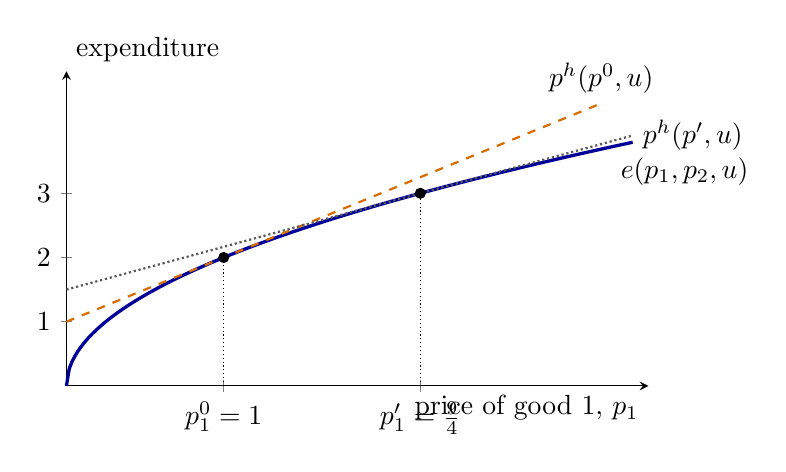
\begin{tikzpicture}
\begin{axis}[
  width=0.74\textwidth, height=0.46\textwidth,
  axis lines=left, xmin=0, xmax=3.7, ymin=0, ymax=4.9,
  xlabel={price of good 1, $p_1$}, ylabel={expenditure},
  xtick={1,2.25}, xticklabels={$p_1^0 = 1$,$p_1' = \frac{9}{4}$},
  ytick={1,2,3}, yticklabels={$1$,$2$,$3$},
  every axis x label/.style={at={(ticklabel* cs:1)}, anchor=north east},
  every axis y label/.style={at={(ticklabel* cs:1)}, anchor=south west},
  clip=false]
\addplot[domain=0:3.6, samples=200, very thick, blue!60!black] {2*sqrt(x)}
  node[pos=0.97, below right, black] {$e(p_1, p_2, u)$};
\addplot[domain=0:3.4, thick, dashed, orange!85!black] {x + 1}
  node[pos=1, above, black] {$p^\T h(p^0, u)$};
\addplot[domain=0:3.6, thick, densely dotted, gray!70!black] {(2/3)*x + 1.5}
  node[pos=1, right, black] {$p^\T h(p', u)$};
\addplot[only marks, mark=*, mark size=1.8pt] coordinates {(1,2) (2.25,3)};
\draw[densely dotted] (axis cs:1,0) -- (axis cs:1,2);
\draw[densely dotted] (axis cs:2.25,0) -- (axis cs:2.25,3);
\end{axis}
\end{tikzpicture}
\caption{Shephard's lemma as a supporting hyperplane. Cobb-Douglas utility
$U = q_1^{\frac{1}{2}}q_2^{\frac{1}{2}}$ with $p_2 = 1$ and $u = 1$ gives $e(p_1, 1, 1) = 2\sqrt{p_1}$, which is
concave in $p_1$. The cost of the fixed bundle $h(p^0, u) = (1, 1)$ is the line $p_1 + 1$. It lies above
$e$ and touches it at $p_1^0 = 1$, so its slope $h_1(p^0, u) = 1$ equals the slope of $e$ there. The dotted
line repeats the construction at $p_1' = \frac{9}{4}$, where $h(p', u) = (\frac{2}{3}, \frac{3}{2})$. The
expenditure function is the lower envelope of all such lines.}\label{fig:B-expfn}
\end{figure}

\begin{proposition}[Roy's identity, \citealp{Roy1947}]\label{prop:B-roy}
Under \cref{ass:B-preferences}, if $v$ is differentiable at $(p, I)$ with $\frac{\partial v}{\partial I} > 0$
and $e(\cdot, u)$ is differentiable at $p$ for $u = v(p, I)$, then
\begin{equation}\label{eq:B-roy}
q_i(p, I) = -\frac{\partial v(p, I)}{\partial p_i}\left[\frac{\partial v(p, I)}{\partial I}\right]^{-1}.
\end{equation}
\end{proposition}

\Cref{prop:05-roy} proves the identity, together with its share form. The proof differentiates the identity
$v(p, e(p, u)) = u$ of \eqref{eq:B-duality-1} with respect to $p_i$, substitutes Shephard's lemma, and
evaluates at $u = v(p, I)$.

Roy's identity is invariant to increasing transformations of $v$, because a transformation multiplies both
derivatives by the same positive factor. \Cref{sec:B-logsum} shows that the Williams-Daly-Zachary theorem is
the discrete-choice version of the identity.

\begin{proposition}[Slutsky equation, \citealp{Slutsky1915}]\label{prop:B-slutsky}
Under \cref{ass:B-preferences} and differentiability of $q$ and $h$, at $u = v(p, I)$,
\begin{equation}\label{eq:B-slutsky}
\frac{\partial q_i(p, I)}{\partial p_j} = \frac{\partial h_i(p, u)}{\partial p_j} - q_j(p, I)\,\frac{\partial q_i(p, I)}{\partial I} .
\end{equation}
In elasticity form, $\varepsilon^h_{ij} = \varepsilon_{ij} + \eta_iw_j$, where
$\varepsilon^h_{ij} = \frac{\partial\ln h_i}{\partial\ln p_j}$ is the Hicksian elasticity.
\end{proposition}

\Cref{prop:05-slutsky}(i) proves the equation by differentiating $h_i(p, u) = q_i(p, e(p, u))$ with respect to
$p_j$ and applying Shephard's lemma. \Cref{prop:05-elast-identities}(a) derives the elasticity form.

The first term on the right of \eqref{eq:B-slutsky} is the \emph{substitution effect}, which holds utility
fixed. The second is the \emph{income effect}, the response to the loss of purchasing power. The remaining
elasticity identities (Engel and Cournot aggregation, homogeneity, symmetry in share form) are derived in
\cref{sec:05-elasticity-identities}.

\begin{proposition}[Slutsky matrix]\label{prop:B-slutsky-matrix}
Suppose $e(\cdot, u)$ is twice continuously differentiable. Then the Slutsky matrix $S(p, u)$ satisfies:
\begin{enumerate}[label=(\roman*)]
\item $S$ is symmetric: $S_{ij} = S_{ji}$.
\item $S$ is negative semidefinite. In particular $S_{ii} \leq 0$.
\item $Sp = 0$ and $p^\T S = 0$. Hence $S$ has rank at most $n - 1$.
\end{enumerate}
\end{proposition}

\begin{proof}
By Shephard's lemma, $S$ is the Hessian of $e(\cdot, u)$. Parts (ii) to (iv) of \cref{prop:05-slutsky} prove
symmetry, negative semidefiniteness and $Sp = 0$ from Young's theorem, concavity and Euler's theorem
(\cref{prop:B-euler}). Symmetry then gives $p^\T S = 0$. The vector $p$ is nonzero and lies in the null space,
so the rank of $S$ is at most $n - 1$.
\end{proof}

\begin{corollary}[Net substitutes]\label{cor:B-net-substitutes}
If $n \geq 2$ and $S_{ii} < 0$, then $S_{ij} > 0$ for at least one $j \neq i$. Every good with a strictly
negative compensated own-price effect has at least one net substitute.
\end{corollary}

\begin{proof}
Row $i$ of $Sp = 0$ reads $\sum_{j \neq i}S_{ij}p_j = -S_{ii}p_i > 0$. Since every $p_j > 0$, at least one
$S_{ij}$ with $j \neq i$ must be positive.
\end{proof}

Negative semidefiniteness is the compensated law of demand. It is the only sign restriction that consumer
theory places on demand. Marshallian own-price effects can have either sign, because the income effect in
\eqref{eq:B-slutsky} can dominate.

\begin{example}[Cobb-Douglas duality, continuing \cref{ex:B-cobb-douglas}]\label{ex:B-cd-duality}
Let $U(q) = \prod_iq_i^{a_i}$ with $a_i > 0$ and $\sum_ia_i = 1$. This is an increasing transformation of
$\sum_ia_i\ln q_i$, so Marshallian demand is again $q_i = \frac{a_iI}{p_i}$. Substituting demand into $U$,
\begin{equation*}
v(p, I) = \prod_i\left(\frac{a_iI}{p_i}\right)^{a_i} = I\prod_i\left(\frac{a_i}{p_i}\right)^{a_i}.
\end{equation*}
Setting $v(p, e) = u$ and solving for $e$ gives the expenditure function
\begin{equation*}
e(p, u) = u\prod_i\left(\frac{p_i}{a_i}\right)^{a_i}.
\end{equation*}
It is homogeneous of degree one in $p$ because the exponents sum to one. Shephard's lemma gives
$h_i(p, u) = \frac{\partial e}{\partial p_i} = \frac{a_i}{p_i}e(p, u)$. At $u = v(p, I)$ we have $e = I$, so
$h_i = \frac{a_iI}{p_i} = q_i$, as \eqref{eq:B-duality-2} requires. Roy's identity also recovers demand:
\begin{equation*}
\frac{\partial v}{\partial p_i} = -\frac{a_i}{p_i}v, \qquad \frac{\partial v}{\partial I} = \frac{v}{I},
\qquad -\frac{\partial v}{\partial p_i}\left[\frac{\partial v}{\partial I}\right]^{-1} = \frac{a_iI}{p_i}.
\end{equation*}
For the Slutsky equation with $i \neq j$, the compensated cross effect is
$S_{ij} = \frac{a_i}{p_i}\frac{\partial e}{\partial p_j} = \frac{a_ia_je}{p_ip_j}$, which is symmetric in
$(i, j)$. The Marshallian cross effect is zero, and the income term is
$q_j\frac{\partial q_i}{\partial I} = \frac{a_jI}{p_j}\cdot\frac{a_i}{p_i}$. At $e = I$ the two sides of
\eqref{eq:B-slutsky} agree. The own effect is
$S_{ii} = \frac{a_i}{p_i}\cdot\frac{a_ie}{p_i} - \frac{a_ie}{p_i^2} = -\frac{a_i(1 - a_i)e}{p_i^2} < 0$, and
row $i$ of $Sp$ is $\frac{a_ie}{p_i}\left(\sum_ja_j - 1\right) = 0$.
\end{example}

\begin{example}[PIGLOG preferences, \citealp{DeatonMuellbauer1980a}]\label{ex:B-piglog}
The \emph{PIGLOG} (price-independent generalized logarithmic) class of
\citet[eq.~1, p.~313]{DeatonMuellbauer1980a} has
\begin{equation*}
\ln e(p, u) = (1 - u)\ln a(p) + u\ln b(p).
\end{equation*}
Here $a(p)$ and $b(p)$ are positive and homogeneous of degree one. They are interpreted as the costs of
subsistence ($u = 0$) and bliss ($u = 1$). The share form of Shephard's lemma gives
\begin{equation*}
w_i = \frac{\partial\ln a}{\partial\ln p_i} + u\left(\frac{\partial\ln b}{\partial\ln p_i} - \frac{\partial\ln a}{\partial\ln p_i}\right).
\end{equation*}
Inverting $\ln e(p, u) = \ln I$ gives the indirect utility function
$u = \frac{\ln I - \ln a(p)}{\ln b(p) - \ln a(p)}$. Substituting it into the share equation shows that budget
shares are linear in $\ln I$, with coefficients that depend on prices. The AIDS chooses a translog
$\ln a(p)$ and $\ln b(p) = \ln a(p) + \beta_0\prod_kp_k^{\beta_k}$ \citep[eqs.~2--4]{DeatonMuellbauer1980a}.
\Cref{sec:05-aids} carries out that specialization.
\end{example}

\subsection{Integrability and recovering preferences from demand}\label{sec:B-integrability}

Demand is usually estimated before anything is known about preferences. Two questions follow. Is the
estimated system generated by some utility function? If so, can we recover the expenditure function from
it, so that welfare can be measured exactly? The first question is answered by the integrability theorem.
The second is answered by a differential equation.

\begin{proposition}[Integrability, \citealp{HurwiczUzawa1971}]\label{prop:B-integrability}
Let $q(p, I)$ be continuously differentiable on $\R^n_{++} \times \R_{++}$. Suppose it satisfies adding up,
$p^\T q(p, I) = I$, and homogeneity of degree zero in $(p, I)$. Suppose also that the matrix with elements
$S_{ij} = \frac{\partial q_i}{\partial p_j} + q_j\frac{\partial q_i}{\partial I}$ is symmetric and negative
semidefinite at every $(p, I)$. Then, under regularity conditions, there is an increasing and
quasi-concave utility function whose Marshallian demand is $q$.
\end{proposition}

We omit the proof. Its logic is short. We look for a function $e(p, u)$ that satisfies the
system of partial differential equations
\begin{equation}\label{eq:B-integrability-pde}
\frac{\partial e(p, u)}{\partial p_i} = q_i\big(p, e(p, u)\big), \qquad i = 1, \dots, n,
\end{equation}
which combines Shephard's lemma with \eqref{eq:B-duality-2}. Differentiate the $i$-th equation with respect
to $p_j$:
\begin{equation*}
\frac{\partial^2e}{\partial p_j\partial p_i} = \frac{\partial q_i}{\partial p_j} + \frac{\partial q_i}{\partial I}\cdot\frac{\partial e}{\partial p_j}
= \frac{\partial q_i}{\partial p_j} + \frac{\partial q_i}{\partial I}\,q_j = S_{ij}.
\end{equation*}
Mixed partial derivatives must be equal, so a solution can exist only if $S_{ij} = S_{ji}$. This is the
integrability condition of \citet[eqs.~5.2--5.3, p.~50]{DeatonMuellbauer1980b}. Frobenius's
theorem says that symmetry is also sufficient for a local solution. Negative semidefiniteness then makes
the solution concave in $p$, so it is a valid expenditure function
\citep[ch.~3]{MasColellWhinstonGreen1995}. The practical message is that an estimated demand system which
satisfies the four restrictions supports exact welfare analysis (\cref{ch:aids}).

When only one price changes, \eqref{eq:B-integrability-pde} reduces to an ordinary differential equation.
This is the method of \citet{Hausman1981}. Fix the other prices $p_{-1}$ and, for each utility level $u$,
let $\tilde e_u(p_1) = e(p_1, p_{-1}, u)$. Shephard's lemma and \eqref{eq:B-duality-2} give
\begin{equation}\label{eq:B-hausman-ode}
\frac{\dd\tilde e_u(p_1)}{\dd p_1} = h_1(p_1, p_{-1}, u) = q_1\big(p_1, p_{-1}, \tilde e_u(p_1)\big).
\end{equation}
The right side is known once $q_1$ has been estimated, so \eqref{eq:B-hausman-ode} is a first-order
differential equation in the scalar $\tilde e_u$. Each solution curve is one indifference level. We label
the curve by its initial condition. The curve through $(p_1^0, I^0)$ belongs to the utility level
$u^0 = v(p_1^0, p_{-1}, I^0)$, so $\tilde e_{u^0}(p_1^0) = I^0$. If $q_1$ is Lipschitz in income, that is,
$|q_1(p, I) - q_1(p, I')| \leq K|I - I'|$ for a constant $K$, the Picard-Lindel\"of theorem gives a unique solution. Its standard proof is a contraction argument
(\cref{thm:B-banach}). The labeling of utility is arbitrary because utility is ordinal. Money measures such as
the compensating variation do not depend on it.

\citet{Hausman1981} solves \eqref{eq:B-hausman-ode} in closed form for common parametric demands.
\citet[eq.~3, p.~212]{Hausman1997} uses the solution as the ``(partial) expenditure function'' that values a
new cereal brand. The word partial reflects that only the new good's price varies. Under the usual
separability assumptions only the demand curve of the new good needs to be estimated \citep[fn.~7]{Hausman1997}.

\begin{example}[Exact welfare from linear demand]\label{ex:B-hausman-linear}
Let the demand for good 1 be linear in its own price and income,
\begin{equation*}
q_1 = c_0 + c_1p_1 + c_2I, \qquad c_1 < 0,\ c_2 \neq 0,
\end{equation*}
with the other prices fixed and absorbed in $c_0$. Equation \eqref{eq:B-hausman-ode} becomes the linear
equation
\begin{equation*}
\frac{\dd e}{\dd p_1} = c_0 + c_1p_1 + c_2e .
\end{equation*}
\textit{Homogeneous part.} The equation $\frac{\dd e}{\dd p_1} = c_2e$ has the solutions $Ke^{c_2p_1}$ for any
constant $K$.

\textit{Particular solution.} Try $e = A + Bp_1$. Substituting gives $B = c_0 + c_1p_1 + c_2A + c_2Bp_1$ for
all $p_1$. Matching the coefficients on $p_1$ gives $0 = c_1 + c_2B$, so $B = -\frac{c_1}{c_2}$. Matching the
constants gives $B = c_0 + c_2A$, so
\begin{equation*}
A = \frac{B - c_0}{c_2} = -\frac{1}{c_2}\left(c_0 + \frac{c_1}{c_2}\right).
\end{equation*}

\textit{General solution.} Adding the two parts and using the constant of integration as the utility index,
\begin{equation}\label{eq:B-hausman-e}
e(p_1, u) = u\,e^{c_2p_1} - \frac{1}{c_2}\left(c_0 + c_1p_1 + \frac{c_1}{c_2}\right).
\end{equation}
To verify, differentiate: $\frac{\partial e}{\partial p_1} = c_2u\,e^{c_2p_1} - \frac{c_1}{c_2}$. The right
side of the differential equation is
$c_0 + c_1p_1 + c_2u\,e^{c_2p_1} - \left(c_0 + c_1p_1 + \frac{c_1}{c_2}\right)$, which is the same. Inverting
$e(p_1, u) = I$ gives the indirect utility function
\begin{equation*}
v(p_1, I) = e^{-c_2p_1}\left[I + \frac{1}{c_2}\left(c_0 + c_1p_1 + \frac{c_1}{c_2}\right)\right],
\end{equation*}
and Roy's identity returns $q_1$. The Hicksian demand is
$h_1(p_1, u) = c_2u\,e^{c_2p_1} - \frac{c_1}{c_2}$.

\textit{Compensating variation of a price change.} Let the price rise from $p_1^0$ to $p_1^0 + \Delta$ at income
$I^0$, and write $q^0 = c_0 + c_1p_1^0 + c_2I^0$ for initial demand. The initial utility satisfies
$u^0e^{c_2p_1^0} = I^0 + \frac{1}{c_2}\left(c_0 + c_1p_1^0 + \frac{c_1}{c_2}\right) = \frac{q^0}{c_2} + \frac{c_1}{c_2^2}$.
Substituting into $CV = e(p_1^0 + \Delta, u^0) - I^0$ and collecting terms,
\begin{equation}\label{eq:B-hausman-cv}
CV = \left(\frac{q^0}{c_2} + \frac{c_1}{c_2^2}\right)\left(e^{c_2\Delta} - 1\right) - \frac{c_1}{c_2}\Delta .
\end{equation}
Expanding $e^{c_2\Delta}$ to third order shows that $CV \to q^0\Delta + \frac{c_1}{2}\Delta^2$ as $c_2 \to 0$. The
limit is the Marshallian surplus loss $\int_{p_1^0}^{p_1^0 + \Delta}(c_0 + c_1t + c_2I^0)\,\dd t$. Without income
effects the two measures coincide.

\textit{Virtual price and the value of the good.} The virtual price $p_1^V$ is the price at which compensated
demand falls to zero (\cref{def:B-virtual}). The Hicksian slope at the initial point is
$\frac{\partial h_1}{\partial p_1} = c_1 + c_2q^0$, the Slutsky term. Negativity requires $c_1 + c_2q^0 \leq 0$, and we
assume the strict inequality. Setting
$h_1(p_1^V, u^0) = 0$ and using the expression for $u^0$ gives
\begin{equation*}
e^{c_2(p_1^V - p_1^0)} = \frac{c_1}{c_1 + c_2q^0},
\qquad\text{so}\qquad
p_1^V - p_1^0 = \frac{1}{c_2}\ln\frac{c_1}{c_1 + c_2q^0} .
\end{equation*}
Substituting $\Delta = p_1^V - p_1^0$ into \eqref{eq:B-hausman-cv}, the first term becomes
$\frac{c_2q^0 + c_1}{c_2^2}\cdot\frac{-c_2q^0}{c_1 + c_2q^0} = -\frac{q^0}{c_2}$. The compensating variation of
removing the good is therefore
\begin{equation*}
CV^V = -\frac{q^0}{c_2} - \frac{c_1}{c_2^2}\ln\frac{c_1}{c_1 + c_2q^0} .
\end{equation*}
As $c_2 \to 0$, $p_1^V - p_1^0 \to -\frac{q^0}{c_1}$, the Marshallian choke price, and $CV^V \to \frac{(q^0)^2}{2|c_1|}$,
the Marshallian triangle. For a numerical illustration take $c_0 = 4$, $c_1 = -2$, $c_2 = 0.01$, $I^0 = 100$
and $p_1^0 = 1$. Then $q^0 = 3$, the budget share is 3 percent and the income elasticity is $\frac{1}{3}$. The
Hicksian virtual price is $2.511$, against a Marshallian choke price of $2.5$. The exact value of the good
is $CV^V = 2.273$, about 1 percent above the Marshallian triangle of $2.25$. Doubling the price costs
$CV = 2.012$, against a Marshallian loss of $2$. For a normal good the exact measure exceeds the Marshallian
one, as \cref{prop:05-cv-ordering} predicts, and the gap is small when the good is a small part of the
budget \citep{Willig1976}.
\end{example}

\subsection{Welfare measures and virtual prices}\label{sec:B-welfare}

\begin{definition}[Compensating and equivalent variation]\label{def:B-cv-ev}
Let prices change from $p^0$ to $p^1$ at fixed income $I$, and let $u^0 = v(p^0, I)$ and $u^1 = v(p^1, I)$.
The \emph{compensating variation} and the \emph{equivalent variation} are
\begin{equation}\label{eq:B-cv-ev}
CV = e(p^1, u^0) - I, \qquad EV = I - e(p^0, u^1).
\end{equation}
This is \cref{def:05-cv-ev}. With these signs both measures are positive for a welfare loss.
\end{definition}

The CV is the extra income that restores the old utility at the new prices. The EV is the income the
consumer would give up at the old prices to be as badly off as after the change. \Cref{sec:05-cv-ev} uses
Shephard's lemma to write each measure as an area to the left of a Hicksian demand curve,
\begin{equation}\label{eq:B-cv-integral}
CV = \int_{p_i^0}^{p_i^1}h_i(t, p_{-i}, u^0)\,\dd t, \qquad EV = \int_{p_i^0}^{p_i^1}h_i(t, p_{-i}, u^1)\,\dd t ,
\end{equation}
when only $p_i$ changes. When several prices change, the CV is a line integral of Hicksian demands that does not
depend on the path \eqref{eq:05-cv-path}. For a normal good the Marshallian surplus lies between $EV$ and $CV$
(\cref{prop:05-cv-ordering}).

\Cref{def:B-cv-ev} follows \citet[Section~7.4, eqs.~4.1--4.2, p.~186]{DeatonMuellbauer1980b}, who also
sign both measures so that they are positive for a loss. Two bounds use only observed prices and
quantities. Let $q^0 = q(p^0, I)$ and $q^1 = q(p^1, I)$ be the bundles chosen before and after the change.
The old bundle reaches $u^0$ and costs $p^{1\T}q^0$ at the new prices, so $e(p^1, u^0) \leq p^{1\T}q^0$. The
new bundle reaches $u^1$ and costs $p^{0\T}q^1$ at the old prices, so $e(p^0, u^1) \leq p^{0\T}q^1$. Since
$I = p^{0\T}q^0 = p^{1\T}q^1$,
\begin{equation}\label{eq:B-cv-ev-bounds}
CV \leq q^{0\T}(p^1 - p^0), \qquad EV \geq q^{1\T}(p^1 - p^0).
\end{equation}
The Laspeyres variation $q^{0\T}(p^1 - p^0)$ overstates the compensation the consumer needs. The Paasche
variation $q^{1\T}(p^1 - p^0)$ understates the equivalent loss. To first order in $p^1 - p^0$ both bounds hold with equality
(their eq.~4.3, p.~187). The ratio forms of the same objects are \emph{true cost-of-living indices}. At a
reference utility $u^R$ the index is
\begin{equation*}
\mathrm{COL}(p^1, p^0; u^R) = \frac{e(p^1, u^R)}{e(p^0, u^R)}
\end{equation*}
(their Section~7.1, eq.~1.2, p.~170). The argument behind \eqref{eq:B-cv-ev-bounds} bounds
$\mathrm{COL}(p^1, p^0; u^0)$ above by the Laspeyres index $\frac{p^{1\T}q^0}{p^{0\T}q^0}$. It bounds
$\mathrm{COL}(p^1, p^0; u^1)$ below by the Paasche index $\frac{p^{1\T}q^1}{p^{0\T}q^1}$ (their eqs.~1.3--1.4,
p.~172).

A new good, or a good that disappears, is a price change of a special kind. The good is absent in one
of the two situations. \citet{Hicks1940} proposed to treat the missing good as available at a price
that would ``just make the demands for these commodities (from the whole community) equal to zero.''
The passage is on p.~144 and is quoted by \citet[p.~211]{Hausman1997}. \citet{Rothbarth1941} called such prices the virtual price
system.

\begin{definition}[Virtual price]\label{def:B-virtual}
Given the other prices $p_{-i}$ and the utility level $u$, the \emph{virtual} (reservation) \emph{price} of
good $i$ is the lowest $p_i^V$ with $h_i(p_i^V, p_{-i}, u) = 0$, as in \cref{def:05-virtual}. If $h_i > 0$ at
every finite price, we set $p_i^V = \infty$.
\end{definition}

\citet[eqs.~1--2, p.~211]{Hausman1997} writes the condition with the Marshallian demand,
$0 = g(p_1, \dots, p_{n-1}, p_n^*, y)$. He then replaces income by the expenditure function at the
post-introduction utility, so that the virtual price is computed on the Hicksian demand (his footnote 5).

\begin{proposition}[Valuing the removal of a good]\label{prop:B-virtual}
Let $e_{-i}(p_{-i}, u) = \min\{p_{-i}^\T q_{-i} : U(0, q_{-i}) \geq u\}$ be the expenditure function when good
$i$ is unavailable. Under \cref{ass:B-preferences}:
\begin{enumerate}[label=(\roman*)]
\item $e(p_i, p_{-i}, u) \leq e_{-i}(p_{-i}, u)$ for every $p_i$, and $e$ is nondecreasing in $p_i$.
\item If $p_i^V < \infty$, then $e(p_i^V, p_{-i}, u) = e_{-i}(p_{-i}, u)$.
\item If $p_i^V = \infty$, then $e(p_i, p_{-i}, u) \to e_{-i}(p_{-i}, u)$ as $p_i \to \infty$.
\item In both cases the compensating variation of removing good $i$ at prices $p^0$ is
\begin{equation}\label{eq:B-cv-removal}
CV = e_{-i}(p_{-i}^0, u^0) - e(p^0, u^0) = \int_{p_i^0}^{p_i^V}h_i(t, p_{-i}^0, u^0)\,\dd t .
\end{equation}
\end{enumerate}
\end{proposition}

\begin{proof}
Parts (i) and (ii) are \cref{prop:05-removal}, and monotonicity is \cref{prop:B-e-properties}. (iii) By (i)
the limit $L$ exists and $L \leq e_{-i}$. Write $h(p_i)$ for $h(p_i, p_{-i}, u)$. Since
$p_ih_i(p_i) \leq e(p_i, p_{-i}, u) \leq e_{-i}$, we have $h_i(p_i) \to 0$. The bundles $h(p_i)$ are bounded, so a
subsequence converges to some $\bar q$ with $\bar q_i = 0$ and, by continuity of $U$, $U(\bar q) \geq u$. Then
$e_{-i} \leq p_{-i}^\T\bar q_{-i} = \lim p_{-i}^\T h_{-i}(p_i) \leq L$. (iv) Combine (ii) or (iii) with Shephard's lemma
and the fundamental theorem of calculus.
\end{proof}

\begin{remark}[Rationing and shadow prices]\label{rem:B-rationing}
Virtual prices are a special case of the theory of rationing in \citet[Section~4.3,
pp.~109--114]{DeatonMuellbauer1980b}. Suppose the consumer must buy exactly $z$ units of good $i$, and let
$e^*(p, u, z) = \min_q\{p^\T q : U(q) \geq u,\ q_i = z\}$ be the \emph{restricted expenditure function}. The
\emph{shadow price} $p_i^*(p_{-i}, u, z)$ is the price at which the consumer would choose $z$ freely, so
$h_i(p_i^*, p_{-i}, u) = z$. \Cref{sec:05-welfare-virtual} derives two identities, their eqs.~3.12 and 3.7
(pp.~112--114):
\begin{equation*}
e^*(p, u, z) = e(p_i^*, p_{-i}, u) + (p_i - p_i^*)z,
\qquad
\frac{\partial e^*}{\partial z} = p_i - p_i^* .
\end{equation*}
A marginal unit of the ration costs $p_i$, and it saves $p_i^*$ of spending on other goods at constant
utility. Their Figure~4.6 (p.~113) reads $p_i^*$ off the tangent to the indifference curve at the rationed
bundle. An unavailable good is the ration $z = 0$. When the virtual price of \cref{def:B-virtual} is finite, it
is the shadow price of this ration. The first identity then gives $e^*(p, u, 0) = e(p_i^V, p_{-i}, u)$, which is
part (ii) of \cref{prop:B-virtual}. Integrating $\frac{\partial e^*}{\partial z}$ from $0$ to $z^0 = h_i(p^0, u^0)$
gives
\begin{equation*}
CV = e^*(p^0, u^0, 0) - e^*(p^0, u^0, z^0) = \int_0^{z^0}\big[p_i^*(p_{-i}^0, u^0, z) - p_i^0\big]\,\dd z .
\end{equation*}
The integrand is the inverse compensated demand curve minus the price. The integral is therefore the area
of \eqref{eq:B-cv-removal}, measured along the quantity axis. Cross derivatives of $e^*$ give symmetry
results for shadow prices that parallel Slutsky symmetry (their eqs.~3.8--3.10, pp.~113--114).
\Cref{rem:B-lechatelier} uses the restricted demands to show that a ration dampens the compensated
price responses of the other goods.
\end{remark}

The ratio $\frac{e(p_i^V, p_{-i}, u^0)}{e(p^0, u^0)}$ is the exact cost-of-living index that corrects for the
availability of the good \citep[eq.~4, p.~212]{Hausman1997}. It is $\mathrm{COL}$ at $u^R = u^0$, with the
price of good $i$ raised to its virtual price. Hausman labels the period in which the good is available as
period~1. He therefore evaluates the index at the post-introduction utility $u^1$, as $\frac{y^*}{y}$ with
$y^* = e(p_1, \dots, p_{n-1}, p_n^*, u^1)$. Our $u^0$ is the utility when the good is available, so the two
ratios coincide. The value of a good is the area under its
compensated demand curve from the actual price up to the virtual price. Functional form therefore matters a
great deal. In the AIDS a budget share reaches zero at a finite log price, so the virtual price is finite
and depends on the estimated own and cross effects (\cref{ch:aids}). In the CES and logit models demand is
positive at every finite price, so $p_i^V = \infty$. For the CES, the expenditure function is
$e(p, u) = P(p)\,u$ with $P(p)^{1 - \sigma_{\mathrm{CES}}} = \sum_ja_jp_j^{1 - \sigma_{\mathrm{CES}}}$ and
$\sigma_{\mathrm{CES}} > 1$. Removing good $i$ gives
\begin{equation*}
P_{-i}^{1 - \sigma_{\mathrm{CES}}} = P^{1 - \sigma_{\mathrm{CES}}} - a_ip_i^{1 - \sigma_{\mathrm{CES}}}
= P^{1 - \sigma_{\mathrm{CES}}}(1 - w_i),
\end{equation*}
where $w_i = a_i\left(\frac{p_i}{P}\right)^{1 - \sigma_{\mathrm{CES}}}$ is the budget share. Since $e$ is linear in $P$,
\begin{equation*}
\frac{CV}{I} = \frac{P_{-i}}{P} - 1 = (1 - w_i)^{\frac{1}{1 - \sigma_{\mathrm{CES}}}} - 1 > 0 .
\end{equation*}
The logit analogue is $-\frac{1}{\alpha}\ln(1 - s_i)$ per consumer (\cref{prop:B-cs}). In both models the loss
depends only on the share and one substitution parameter. The value of variety is built into the
functional form. \citet[p.~210]{Hausman1997} instead estimates a flexible demand system for cereal and finds
a virtual price for Apple-Cinnamon Cheerios about twice its actual price (\cref{ch:newgoods}).

\begin{proposition}[Quasi-linear utility]\label{prop:B-quasilinear}
Let there be a numeraire good $0$ with price one, and let $U(q_0, q) = q_0 + \tilde u(q)$ with
$q \in \R^n_+$. The function $\tilde u$ is twice continuously differentiable and strictly increasing, with a
negative definite Hessian (hence strictly concave).
Suppose the solution is interior, with $q_0 > 0$ and $q \gg 0$. Then:
\begin{enumerate}[label=(\roman*)]
\item Marshallian demand $q(p)$ for goods $1, \dots, n$ solves $\nabla\tilde u(q) = p$ and does not depend on
  income, so $\frac{\partial q_i}{\partial I} = 0$ for $i \geq 1$.
\item $v(p, I) = I + CS(p)$ and $e(p, u) = u - CS(p)$, where $CS(p) = \max_q\{\tilde u(q) - p^\T q\}$.
\item Hicksian and Marshallian demands coincide, $h(p, u) = q(p)$, and the Slutsky matrix equals
  $\frac{\partial q}{\partial p^\T} = [D^2\tilde u(q)]^{-1}$.
\item For any change from $p^0$ to $p^1$,
\begin{equation}\label{eq:B-quasilinear-cv}
CV = EV = CS(p^0) - CS(p^1) = \int_0^1\sum_{i=1}^nq_i(p(t))\,\dot p_i(t)\,\dd t,
\end{equation}
  the change in Marshallian consumer surplus, along any path $p(t)$ from $p^0$ to $p^1$.
\end{enumerate}
\end{proposition}

\begin{proof}
(i) Substitute the budget constraint $q_0 = I - p^\T q$ into utility. The consumer maximizes
$I - p^\T q + \tilde u(q)$ over $q$. The first-order conditions are $\frac{\partial\tilde u}{\partial q_i} = p_i$,
and strict concavity makes the solution unique. Income does not appear. (ii) Substituting the solution,
$v(p, I) = I - p^\T q(p) + \tilde u(q(p)) = I + CS(p)$. Setting $v(p, e) = u$ and solving gives
$e = u - CS(p)$. (iii) By the envelope theorem, $\frac{\partial CS}{\partial p_i} = -q_i(p)$. Shephard's lemma then
gives $h_i = \frac{\partial e}{\partial p_i} = q_i(p)$. Differentiating the identity $\nabla\tilde u(q(p)) = p$ gives
$D^2\tilde u\cdot\frac{\partial q}{\partial p^\T} = I_n$, where $I_n$ is the identity matrix. (iv) From (ii),
\begin{align*}
CV &= e(p^1, u^0) - e(p^0, u^0) = CS(p^0) - CS(p^1), \\
EV &= e(p^0, u^0) - e(p^0, u^1) = u^0 - u^1 = CS(p^0) - CS(p^1).
\end{align*}
The line integral follows from $\nabla CS = -q$ and the fundamental theorem of calculus. It is path
independent because $q$ is a gradient.
\end{proof}

\Cref{prop:B-quasilinear} is the reason why welfare in discrete-choice models with utility linear in income
is exact. There the utility of alternative $j$ is $\alpha(y_i - p_j) + \tilde\delta_j + \epsilon_{ij}$, and every
alternative has the same marginal utility of income $\alpha$. The expected surplus formula of
\cref{prop:B-cs} therefore measures $CV$ and $EV$ at once (\cref{ch:logit}, \cref{ch:newgoods}). The interiority
condition $q_0 > 0$ matters. If the numeraire hits zero, income effects reappear.

\begin{remark}[Income effects in discrete choice]\label{rem:B-income-effects}
With income effects, for example utility $\alpha\ln(y_i - p_j)$ as in random-coefficients models of car demand,
the marginal utility of income depends on the alternative chosen. The expected maximum utility is then not
a money measure, and the compensating variation has no closed form. It must be computed consumer by
consumer, by solving for the income that restores each consumer's expected utility (\cref{ch:newgoods}).
\end{remark}

\begin{remark}[Aggregation]\label{rem:B-gorman}
Suppose we want a representative consumer whose expenditure function is the sum of the individual
ones, for every distribution of income. This is possible if and only if individual expenditure functions
have the \emph{Gorman polar form} $e_h(p, u_h) = a_h(p) + b(p)u_h$ with a common $b(p)$
\citep{Gorman1953, Gorman1961}. Roy's identity gives individual demands
$q_i^h = \frac{\partial a_h}{\partial p_i} + \frac{\partial\ln b}{\partial p_i}\,(I_h - a_h(p))$, so every household has the same
marginal propensity to spend on good $i$, and aggregate demand depends only on total income. Quasi-linear
preferences are of Gorman form, with $a_h(p) = -CS_h(p)$ and $b(p) = 1$. This is why consumer surplus can be
summed across consumers in discrete-choice welfare analysis.

\citet[Section~6.1, pp.~149--153]{DeatonMuellbauer1980b} reach the Gorman form from the demand side.
Average demand depends only on average expenditure if and only if Engel curves are linear with slopes
common to all households (their eq.~1.4, p.~150). With utility maximization this forces the Gorman polar
form (their eq.~1.6, p.~151). Their Section~6.2 (pp.~154--157) aggregates budget shares instead. Let there be
$H$ households, write $\bar I$ for mean income and $\omega_h = \frac{I_h}{H\bar I}$ for household $h$'s share of
total income. The aggregate budget share is the income-weighted mean $\bar w_i = \sum_h\omega_hw_i^h$ (their
eq.~2.1). Under PIGLOG preferences common to all households, \cref{ex:B-piglog} gives
$w_i^h = A_i(p) + B_i(p)\ln I_h$, with coefficients that depend only on prices. Hence
\begin{equation*}
\bar w_i = A_i(p) + B_i(p)\ln I_0, \qquad \ln I_0 = \sum_h\omega_h\ln I_h .
\end{equation*}
A single consumer with the \emph{representative income} $I_0$ reproduces the aggregate shares. Substitute
$I_h = \omega_hH\bar I$ and use $\sum_h\omega_h = 1$:
\begin{equation*}
\ln I_0 = \ln\bar I + \ln H + \sum_h\omega_h\ln\omega_h = \ln\bar I + \ln H - \ln Z,
\end{equation*}
where $\ln Z = -\sum_h\omega_h\ln\omega_h$ is Theil's entropy of the income shares, which
\citet[p.~157]{DeatonMuellbauer1980b} call an entropy measure of dispersion. So $I_0 = \frac{H}{Z}\bar I$,
their eq.~2.15 (p.~157). The index $Z$ reaches its maximum $H$ when all incomes are equal. Representative
income therefore exceeds mean income whenever incomes differ, and it moves with the distribution of income.
The wider class of \emph{price-independent generalized linear} (PIGL) preferences gives a similar formula
(their eqs.~2.7--2.13). \Cref{sec:05-gorman,sec:05-pigl} prove
these results and apply them to the AIDS.
\end{remark}

\subsection{Producer duality}\label{sec:B-producer}

The firm's problems have the same structure as the consumer's, with one simplification: there are no
income effects. A single-output firm has a production function $\varphi : \R^L_+ \to \R_+$, which is
continuous and increasing. It buys inputs $x = (x_1, \dots, x_L)$ at prices $r \in \R^L_{++}$ and sells output at
price $p > 0$. (Here $r$ is an input price vector, not a reserve price.) The \emph{profit function} and the
\emph{cost function} are
\begin{equation}\label{eq:B-profit-cost}
\pi(p, r) = \max_{x \geq 0}\big\{p\varphi(x) - r^\T x\big\},
\qquad
C(r, q) = \min_{x \geq 0}\big\{r^\T x : \varphi(x) \geq q\big\}.
\end{equation}
We assume that the profit maximum exists and is attained at a unique input vector $x^*(p, r)$, with supply
$q^*(p, r) = \varphi(x^*(p, r))$. This requires decreasing returns at large scale. The cost minimizer is the
vector of \emph{conditional factor demands} $x(r, q)$.

\begin{proposition}[Profit function and Hotelling's lemma, \citealp{Hotelling1932}]\label{prop:B-profit-fn}
The profit function has the following properties.
\begin{enumerate}[label=(\roman*)]
\item It is homogeneous of degree one in $(p, r)$.
\item It is convex in $(p, r)$, nondecreasing in $p$ and nonincreasing in $r$.
\item Where it is differentiable, $\frac{\partial\pi}{\partial p} = q^*(p, r)$ and
  $\frac{\partial\pi}{\partial r_\ell} = -x^*_\ell(p, r)$.
\item Where it is twice continuously differentiable, $\frac{\partial q^*}{\partial p} \geq 0$,
  $\frac{\partial x^*_\ell}{\partial r_\ell} \leq 0$, $\frac{\partial x^*_\ell}{\partial r_m} = \frac{\partial x^*_m}{\partial r_\ell}$
  and $\frac{\partial q^*}{\partial r_\ell} = -\frac{\partial x^*_\ell}{\partial p}$.
\end{enumerate}
\end{proposition}

\begin{proof}
(i) Scaling $(p, r)$ by $\lambda > 0$ scales the objective by $\lambda$ for every $x$. (ii) For each $x$, the map
$(p, r) \mapsto p\varphi(x) - r^\T x$ is linear, and the maximum of linear functions is convex. The
monotonicity is immediate. (iii) Fix $(p^0, r^0)$ and $x^0 = x^*(p^0, r^0)$. For every $(p, r)$,
\begin{equation*}
\pi(p, r) \geq p\varphi(x^0) - r^\T x^0,
\end{equation*}
with equality at $(p^0, r^0)$. The difference between the two sides is minimized at $(p^0, r^0)$, so its
gradient vanishes there. This is the mirror image of the supporting-hyperplane proof of Shephard's lemma
(\cref{prop:05-shephard}).
\Cref{ex:B-hotelling} obtained the same result from the envelope theorem. (iv) The Hessian of $\pi$ is symmetric and positive
semidefinite by convexity. By (iii) its entries are $\frac{\partial^2\pi}{\partial p^2} = \frac{\partial q^*}{\partial p}$,
$\frac{\partial^2\pi}{\partial r_\ell^2} = -\frac{\partial x^*_\ell}{\partial r_\ell}$,
$\frac{\partial^2\pi}{\partial r_\ell\partial r_m} = -\frac{\partial x^*_\ell}{\partial r_m}$ and
$\frac{\partial^2\pi}{\partial p\,\partial r_\ell} = \frac{\partial q^*}{\partial r_\ell}$. Nonnegative diagonal elements and symmetry
give the four statements.
\end{proof}

Supply curves slope up and factor demands slope down for every technology. The consumer analogue holds only
for compensated demand. The difference is the absence of an income effect.

\begin{proposition}[Cost function and Shephard's lemma for costs]\label{prop:B-cost-fn}
The cost function has the following properties.
\begin{enumerate}[label=(\roman*)]
\item It is homogeneous of degree one and concave in $r$, and nondecreasing in $r$ and in $q$.
\item Where it is differentiable in $r$, $x_\ell(r, q) = \frac{\partial C(r, q)}{\partial r_\ell}$.
\item Where the cost minimizer and its multiplier $\mu$ are differentiable,
  $mc(r, q) \equiv \frac{\partial C(r, q)}{\partial q} = \mu(r, q)$.
\item Where $C$ is twice continuously differentiable, $\frac{\partial x_\ell}{\partial r_m} = \frac{\partial x_m}{\partial r_\ell}$,
  the matrix $\left[\frac{\partial x_\ell}{\partial r_m}\right]$ is negative semidefinite, and
  $\sum_mr_m\frac{\partial x_\ell}{\partial r_m} = 0$.
\end{enumerate}
\end{proposition}

\begin{proof}
The cost function is the expenditure function with $U$ replaced by $\varphi$, $u$ by $q$ and $p$ by $r$. The
proofs of \cref{prop:05-e-properties}, \cref{prop:05-shephard} and \cref{prop:05-slutsky} apply word for word,
which gives (i), (ii) and (iv). Monotonicity in $q$ holds because a higher target shrinks the feasible
set. Part (iii) is \cref{ex:B-shephard-cost}: the partial derivative of the Lagrangian
$r^\T x - \mu[\varphi(x) - q]$ with respect to $q$ is $\mu$, and the envelope theorem with constraints
(\cref{thm:B-envelope-constrained}) gives the result.
\end{proof}

Profit maximization can be done in two steps. First minimize the cost of each output level. Then choose
output to maximize $pq - C(r, q)$. At an interior optimum with $C$ convex in $q$, the second step gives
$p = mc(r, q^*)$, and $\pi(p, r) = \max_q\{pq - C(r, q)\}$.

\begin{remark}[Returns to scale]\label{rem:B-returns}
If $\varphi$ is homogeneous of degree $B > 0$, then $C(r, q) = q^{\frac{1}{B}}C(r, 1)$. To see this, note that
$\varphi(x) \geq 1$ holds if and only if $\varphi(q^{\frac{1}{B}}x) = q\varphi(x) \geq q$. The map
$x \mapsto q^{\frac{1}{B}}x$ is therefore a bijection between the feasible sets for outputs $1$ and $q$, and it
multiplies cost by $q^{\frac{1}{B}}$. Marginal cost is $mc = \frac{1}{B}q^{\frac{1}{B} - 1}C(r, 1)$. It is constant
under constant returns ($B = 1$), rising under decreasing returns ($B < 1$) and falling under increasing
returns ($B > 1$). The ratio of average to marginal cost equals $B$.
\end{remark}

\begin{example}[Fixed proportions]\label{ex:B-leontief}
Let $\varphi(x) = \min_\ell\frac{x_\ell}{b_\ell}$ with input requirements $b_\ell > 0$. Producing $q$ requires
$x_\ell \geq b_\ell q$ for every $\ell$. Any excess input raises cost because $r \gg 0$, so the cost minimizer is
$x_\ell(r, q) = b_\ell q$ and
\begin{equation*}
C(r, q) = q\sum_{\ell = 1}^Lb_\ell r_\ell, \qquad mc = \sum_{\ell = 1}^Lb_\ell r_\ell .
\end{equation*}
Shephard's lemma holds, $\frac{\partial C}{\partial r_\ell} = b_\ell q = x_\ell$, although $\varphi$ is not
differentiable. Only the differentiability of $C$ matters, as in the supporting-hyperplane proof of
\cref{prop:05-shephard}.
Conditional factor demands do not respond to input prices, so the substitution matrix is zero. Marginal
cost is constant in output and linear in input prices. Suppose one input is a raw material with requirement
$k$ per unit of output and price $p^{\mathrm{raw}}$, and the other inputs cost $c_0$ per unit of output. Then
$mc = c_0 + k\,p^{\mathrm{raw}}$, the form of a refiner's marginal cost used in \cref{ch:conduct}.
\end{example}

Flexible cost functions play the role in production that flexible expenditure functions play in demand.
The translog cost function of \citet{ChristensenJorgensonLau1973} specifies $\ln C(r, q)$ as a second-order
polynomial in $\ln r$ and $\ln q$. Shephard's lemma in share form gives the cost shares
$w^C_\ell = \frac{\partial\ln C}{\partial\ln r_\ell} = a_\ell + \sum_m\gamma_{\ell m}\ln r_m + \gamma_{\ell q}\ln q$, which are
linear in logs like the AIDS share equations. Homogeneity of degree one in $r$ requires
$\sum_\ell a_\ell = 1$ and $\sum_\ell\gamma_{\ell m} = \sum_\ell\gamma_{\ell q} = 0$. Network cost functions with hub
economies, as in \cref{ch:airlines}, are built in the same spirit. \Cref{tab:B-duality} collects the four
problems of this section.

\begin{table}[htbp]
\centering
\caption{Four optimization problems and their value functions}\label{tab:B-duality}
\footnotesize
\begin{tabularx}{\textwidth}{@{}>{\raggedright\arraybackslash}X l l l l@{}}
\toprule
Problem & Value & Homogeneity & Curvature & Derivative identity \\
\midrule
UMP: $\max_q\{U(q) : p^\T q \leq I\}$ & $v(p, I)$ & degree 0 in $(p, I)$ & quasi-convex in $p$ &
  Roy: $q_i = -\frac{\partial v}{\partial p_i}\left[\frac{\partial v}{\partial I}\right]^{-1}$ \\[5pt]
EMP: $\min_q\{p^\T q : U(q) \geq u\}$ & $e(p, u)$ & degree 1 in $p$ & concave in $p$ &
  Shephard: $h_i = \frac{\partial e}{\partial p_i}$, $w_i = \frac{\partial\ln e}{\partial\ln p_i}$ \\[5pt]
Profit: $\max_x\{p\varphi(x) - r^\T x\}$ & $\pi(p, r)$ & degree 1 in $(p, r)$ & convex in $(p, r)$ &
  Hotelling: $q^* = \frac{\partial\pi}{\partial p}$, $x^*_\ell = -\frac{\partial\pi}{\partial r_\ell}$ \\[5pt]
Cost: $\min_x\{r^\T x : \varphi(x) \geq q\}$ & $C(r, q)$ & degree 1 in $r$ & concave in $r$ &
  Shephard: $x_\ell = \frac{\partial C}{\partial r_\ell}$, $mc = \frac{\partial C}{\partial q}$ \\
\bottomrule
\end{tabularx}

\medskip
\begin{minipage}{\textwidth}
\footnotesize Notes: UMP and EMP are the utility maximization and expenditure minimization problems.
Symmetric second derivatives of each value function give Slutsky symmetry (EMP) and the reciprocity
relations $\frac{\partial x_\ell}{\partial r_m} = \frac{\partial x_m}{\partial r_\ell}$ (profit and cost). Curvature
gives the sign restrictions: a negative semidefinite Slutsky matrix, upward-sloping supply and downward-sloping
factor demands.
\end{minipage}
\end{table}

\section{Extreme value distributions and logit algebra}\label{sec:B-ev}

Discrete-choice demand rests on one distributional assumption, the type-I extreme value distribution of
the idiosyncratic taste shock. This section collects everything about that distribution and its
multivariate generalization that \cref{ch:diffprod}, \cref{ch:discrete}, \cref{ch:logit}, \cref{ch:blp},
\cref{ch:airlines}, \cref{ch:newgoods} and \cref{ch:mergers} use. \Cref{ch:discrete} proves the core results:
max-stability, the logit formula, the log-sum, the Williams-Daly-Zachary theorem and the GEV theorem.
\Cref{ch:logit} proves the nested-logit formulas. We restate these results with references to their proofs,
and we prove the remaining results here.

The notation is local to this section. Alternatives are $j = 0, 1, \dots, J$, with $j = 0$ the outside good.
Mean utilities are $\delta_j$, normalized by $\delta_0 = 0$ when an outside good is present. The logit
denominator is $\Lambda = 1 + \sum_{k \geq 1}e^{\delta_k}$, which equals $\sum_{k = 0}^Je^{\delta_k}$ under the
normalization. The expected maximum utility is $\mathcal{W}(\delta) = \E[\max_j(\delta_j + \epsilon_j)]$. Euler's
constant is $\gamma_E \approx 0.5772$. We never write a bare $\gamma$, which denotes AIDS coefficients. The GEV
generating function is $H(y_0, \dots, y_J)$ with $y_j = e^{\delta_j}$, the nesting parameter is $\sigma$, and
$W_0$ is the principal branch of the Lambert function. Elasticities follow the global notation: the own-price
elasticity is a positive number, and cross elasticities are signed.

\subsection{Random utility and choice probabilities}\label{sec:B-rum}

\begin{assumption}[Additive random utility]\label{ass:B-arum}
Consumer $i$ obtains utility $u_{ij} = \delta_j + \epsilon_{ij}$ from alternative $j = 0, \dots, J$ and
chooses the alternative with the highest utility. The vector
$\epsilon_i = (\epsilon_{i0}, \dots, \epsilon_{iJ})$ is independent of $\delta$, has an absolutely continuous
distribution $F$, and has finite means, $\E|\epsilon_{ij}| < \infty$.
\end{assumption}

The \emph{acceptance set} of alternative $j$ is the set of shocks for which $j$ is chosen,
\begin{equation*}
A_j(\delta) = \big\{\epsilon : \delta_j + \epsilon_j \geq \delta_k + \epsilon_k \text{ for all } k\big\}.
\end{equation*}
The choice probability, which equals the market share in a large population of consumers with independent
shocks, is
\begin{equation}\label{eq:B-share-integral}
s_j(\delta) = \Pr\big(\epsilon_i \in A_j(\delta)\big) = \int\indic\{\epsilon \in A_j(\delta)\}\,\dd F(\epsilon).
\end{equation}
A tie between $j$ and $k$ requires $\epsilon_j - \epsilon_k = \delta_k - \delta_j$, a hyperplane of Lebesgue
measure zero. Ties therefore have probability zero under an absolutely continuous $F$, the acceptance sets
overlap only on a null set, and $\sum_{j = 0}^Js_j = 1$. Consumer heterogeneity in tastes is handled by
replacing $\delta_j$ with $\delta_j + \mu_{ij}$ and applying every result conditional on the consumer's type.

\begin{proposition}[Normalizations]\label{prop:B-normalizations}
Under \cref{ass:B-arum}:
\begin{enumerate}[label=(\roman*)]
\item (Location) $s(\delta + c\mathbf{1}) = s(\delta)$ for every scalar $c$.
\item (Scale) The shares generated by the utilities $\lambda\delta_j + \lambda\epsilon_{ij}$ equal those generated by
  $\delta_j + \epsilon_{ij}$ for every $\lambda > 0$.
\end{enumerate}
\end{proposition}

\begin{proof}
(i) Adding $c$ to every $\delta_k$ leaves every inequality defining $A_j$ unchanged. (ii) Multiplying every
utility by $\lambda > 0$ preserves their ranking.
\end{proof}

Location invariance means that only utility differences are identified, so we set $\delta_0 = 0$. Scale
invariance means that the variance of $\epsilon$ must be fixed. In the logit model it is fixed at
$\frac{\pi^2}{6}$. Suppose true utility is $\tilde\delta_j - \alpha^*p_j + b\,\epsilon_{ij}$ with a standard Gumbel
$\epsilon_{ij}$ and an unknown scale $b > 0$. Dividing by $b$ gives an observationally equivalent model with price
coefficient $\alpha = \frac{\alpha^*}{b}$. Estimated coefficients are therefore measured relative to the scale of
the shock. Ratios of coefficients, such as the willingness to pay $\frac{\beta_k}{\alpha}$ for characteristic
$k$, are scale free.

The outside good does more than fix the location. Suppose there were no outside good and all inside
prices rose by the same amount $c$. Every $\delta_j$ would fall by $\alpha c$, and by location invariance no
share would change. Aggregate demand for the category would be perfectly inelastic, and a monopolist owning
every product could raise prices without limit. With an outside good whose utility is fixed at
$\delta_0 = 0$, a common price increase moves consumers out of the market. The outside good also lets a new
product draw consumers from not buying, which welfare analysis of new goods needs. In the data it requires
a definition of the market size $M$, which is an assumption. \Cref{fig:B-epsplane} draws the acceptance sets
with two inside goods.

\begin{figure}[htbp]
\centering
\begin{tikzpicture}[scale=0.95]
  \fill[blue!10] (-3,-3) -- (-1,-3) -- (-1,-0.4) -- (-3,-0.4) -- cycle;
  \fill[orange!14] (-1,-3) -- (3,-3) -- (3,3) -- (2.4,3) -- (-1,-0.4) -- cycle;
  \fill[green!11] (-3,-0.4) -- (-1,-0.4) -- (2.4,3) -- (-3,3) -- cycle;
  \draw[-{Stealth[length=2.2mm]}] (-3.2,0) -- (3.3,0) node[below left] {$\epsilon_{1}$};
  \draw[-{Stealth[length=2.2mm]}] (0,-3.2) -- (0,3.3) node[below left] {$\epsilon_{2}$};
  \draw[very thick] (-1,-3) -- (-1,-0.4);
  \draw[very thick] (-3,-0.4) -- (-1,-0.4);
  \draw[very thick] (-1,-0.4) -- (2.4,3);
  \fill (-1,-0.4) circle (1.6pt);
  \node[anchor=north west, fill=white, inner sep=1.5pt, font=\small] at (-0.95,-0.5) {$(-\delta_1, -\delta_2)$};
  \draw[thick, dashed] (-1.6,-3) -- (-1.6,-0.4);
  \draw[thick, dashed] (-3,-0.4) -- (-1.6,-0.4);
  \draw[thick, dashed] (-1.6,-0.4) -- (1.8,3);
  \draw[-{Stealth[length=2mm]}, thick] (-1.05,-1.6) -- (-1.55,-1.6);
  \node[font=\small] at (-2.1,-1.9) {$j = 0$};
  \node[font=\small] at (1.7,-1.6) {$j = 1$};
  \node[font=\small] at (-1.6,1.7) {$j = 2$};
  \node[font=\scriptsize, anchor=west] at (2.45,3.0) {$\epsilon_2 = \epsilon_1 + \delta_1 - \delta_2$};
\end{tikzpicture}
\caption{Choice regions in the space of taste shocks, with two inside goods and an outside good. The shocks
are measured relative to the outside good, $\epsilon_j \equiv \epsilon_{ij} - \epsilon_{i0}$. The consumer buys nothing in
the lower-left quadrant. She buys good 1 to the right of the vertical boundary and below the 45-degree ray,
and good 2 above the horizontal boundary and above the ray. Each share is the probability mass of its region under the
joint density of the shocks. Raising $\delta_1$ moves the corner to the left (dashed lines), and region 1
grows at the expense of both other regions. The figure uses $\delta_1 = 1$ and $\delta_2 = 0.4$.}\label{fig:B-epsplane}
\end{figure}

\subsection{The Gumbel distribution}\label{sec:B-gumbel}

\begin{definition}[Type-I extreme value distribution]\label{def:B-gumbel}
A random variable has the \emph{type-I extreme value} (or \emph{Gumbel}) distribution $\mathrm{EV}(a, b)$,
with location $a \in \R$ and scale $b > 0$, if its CDF and density are
\begin{equation}\label{eq:B-gumbel}
F(x) = \exp\left(-e^{-\frac{x - a}{b}}\right), \qquad
f(x) = \frac{1}{b}\,e^{-\frac{x - a}{b}}\exp\left(-e^{-\frac{x - a}{b}}\right).
\end{equation}
The \emph{standard} Gumbel distribution has $a = 0$ and $b = 1$, with CDF
$F_{\mathrm{EV}}(\epsilon) = \exp(-e^{-\epsilon})$ and density $e^{-\epsilon}\exp(-e^{-\epsilon})$.
\end{definition}

If $\epsilon$ is standard Gumbel, then $a + b\epsilon \sim \mathrm{EV}(a, b)$. Every fact about $\mathrm{EV}(a, b)$
therefore follows from the standard case.

\begin{lemma}[Gumbel from exponential]\label{lem:B-gumbel-exp}
If $E$ has the unit exponential distribution, $\Pr(E > t) = e^{-t}$ for $t \geq 0$, then $-\ln E$ is standard
Gumbel. If $U$ is uniform on $(0, 1)$, then $-\ln(-\ln U)$ is standard Gumbel.
\end{lemma}

\begin{proof}
For every $x$,
\begin{equation*}
\Pr(-\ln E \leq x) = \Pr(\ln E \geq -x) = \Pr(E \geq e^{-x}) = \exp(-e^{-x}).
\end{equation*}
For the second claim, $-\ln U$ is unit exponential because $\Pr(-\ln U > t) = \Pr(U < e^{-t}) = e^{-t}$. This
is also the probability integral transform (\cref{lem:B-pit}) applied to the inverse CDF
$F_{\mathrm{EV}}^{-1}(u) = -\ln(-\ln u)$.
\end{proof}

\begin{proposition}[Moments and shape]\label{prop:B-gumbel-moments}
Let $\epsilon$ be standard Gumbel. Then $\E[\epsilon] = \gamma_E$, $\Var(\epsilon) = \frac{\pi^2}{6}$, the mode is $0$ and
the median is $-\ln\ln 2 \approx 0.367$. The distribution is skewed to the right, with skewness about
$1.14$. For $\mathrm{EV}(a, b)$ the mean is $a + b\gamma_E$ and the variance is $\frac{b^2\pi^2}{6}$.
\end{proposition}

\begin{proof}
By \cref{lem:B-gumbel-exp} write $\epsilon = -\ln E$. For $t < 1$ the moment generating function is
\begin{equation*}
\E\big[e^{t\epsilon}\big] = \E\big[E^{-t}\big] = \int_0^\infty x^{-t}e^{-x}\,\dd x = \Gamma(1 - t),
\end{equation*}
where $\Gamma$ is the gamma function. We use two standard facts about it, $\Gamma'(1) = -\gamma_E$ and
$\Gamma''(1) = \gamma_E^2 + \frac{\pi^2}{6}$. The first two moments are
\begin{equation*}
\E[\epsilon] = \frac{\dd}{\dd t}\Gamma(1 - t)\Big|_{t = 0} = -\Gamma'(1) = \gamma_E,
\qquad
\E[\epsilon^2] = \Gamma''(1) = \gamma_E^2 + \frac{\pi^2}{6},
\end{equation*}
so $\Var(\epsilon) = \frac{\pi^2}{6}$. The density has derivative $f'(x) = f(x)(e^{-x} - 1)$, which is positive
for $x < 0$ and negative for $x > 0$, so the mode is $0$. The median solves $\exp(-e^{-m}) = \frac{1}{2}$, which
gives $m = -\ln\ln 2$. The skewness equals $\frac{12\sqrt{6}\,\zeta(3)}{\pi^3} \approx 1.14$, where $\zeta$ is the Riemann
zeta function. We state this value without proof. The location and scale results follow from
$a + b\epsilon \sim \mathrm{EV}(a, b)$.
\end{proof}

\begin{remark}[Why ``extreme value'']\label{rem:B-fisher-tippett}
The Gumbel distribution is a limit law for maxima. Let $X_1, \dots, X_n$ be independent unit exponential
draws and $X_{(n:n)}$ their maximum (\cref{sec:B-orderstats}). For $x > -\ln n$,
\begin{equation*}
\Pr\big(X_{(n:n)} - \ln n \leq x\big) = \big(1 - e^{-x - \ln n}\big)^n = \left(1 - \frac{e^{-x}}{n}\right)^n \longrightarrow \exp(-e^{-x}).
\end{equation*}
More generally, the centered and scaled maximum of independent draws from any distribution with
exponential-type tails, the normal included, converges to a Gumbel \citep{FisherTippett1928, Gnedenko1943}.
If the taste shock is read as the best of many independent unobserved attributes, this offers a heuristic
justification. The real attraction of the distribution is the closed forms it delivers.
\end{remark}

\begin{figure}[htbp]
\centering
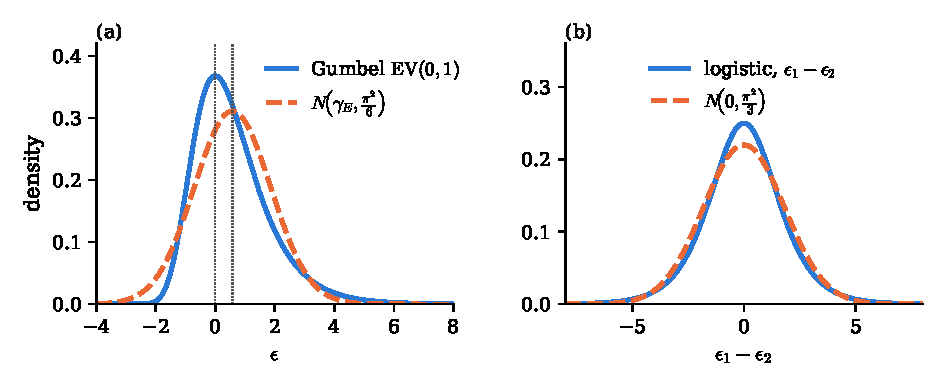
\includegraphics[width=\textwidth]{figures/appB/gumbel_logistic.pdf}
\caption{Panel (a): the standard Gumbel density and the normal density with the same mean $\gamma_E$ and
variance $\frac{\pi^2}{6}$. The dotted lines mark the mode $0$ and the mean $\gamma_E$. The Gumbel is skewed to the
right. Panel (b): the standard logistic density, which is the density of the difference of two independent
standard Gumbels (\cref{prop:B-logistic}), and the normal density with mean $0$ and variance
$\frac{\pi^2}{3}$. The logistic is symmetric and close to the normal, with slightly fatter tails.}\label{fig:B-gumbel}
\end{figure}

\subsection{Max-stability and the logit formula}\label{sec:B-maxstable}

The Gumbel family is closed under maxima with a common scale. This single property delivers the logit
formula, the log-sum and the nested logit.

\begin{proposition}[Max-stability]\label{prop:B-maxstable}
Let $\epsilon_0, \dots, \epsilon_J$ be independent $\mathrm{EV}(0, b)$ and let $\delta_0, \dots, \delta_J$ be constants. Then
\begin{equation}\label{eq:B-maxstable}
\max_j(\delta_j + \epsilon_j) \sim \mathrm{EV}\left(b\ln\sum_{j = 0}^Je^{\frac{\delta_j}{b}},\ b\right).
\end{equation}
\end{proposition}

\Cref{lem:06-maxstable} proves the case $b = 1$, and the text after it extends the proof to scale $b$. The proof
multiplies the independent Gumbel CDFs $\exp(-e^{-\frac{x - \delta_j}{b}})$ and collects the exponents.

\begin{proposition}[Logistic differences]\label{prop:B-logistic}
If $\epsilon_1$ and $\epsilon_2$ are independent standard Gumbels, then $\epsilon_1 - \epsilon_2$ has the standard
logistic distribution,
\begin{equation*}
\Pr(\epsilon_1 - \epsilon_2 \leq x) = \frac{1}{1 + e^{-x}},
\end{equation*}
with density $\frac{e^{-x}}{(1 + e^{-x})^2}$, mean zero and variance $\frac{\pi^2}{3}$.
\end{proposition}

\Cref{lem:06-logistic} proves the result by conditioning on $\epsilon_2$ and substituting $t = e^{-\epsilon_2}$.

\begin{theorem}[Multinomial logit, \citealp{McFadden1974}]\label{thm:B-logit}
Let $u_{ij} = \delta_j + \epsilon_{ij}$ with $\epsilon_{i0}, \dots, \epsilon_{iJ}$ independent standard Gumbels. Then
\begin{equation}\label{eq:B-logit}
s_j(\delta) = \frac{e^{\delta_j}}{\sum_{k = 0}^Je^{\delta_k}} = \frac{e^{\delta_j}}{1 + \sum_{k = 1}^Je^{\delta_k}}
\quad\text{when } \delta_0 = 0 .
\end{equation}
With $\mathrm{EV}(0, b)$ shocks,
\begin{equation*}
s_j(\delta) = \frac{\exp\left(\frac{\delta_j}{b}\right)}{\sum_{k = 0}^J\exp\left(\frac{\delta_k}{b}\right)} .
\end{equation*}
\end{theorem}

\citet[eqs.~3.14--3.15, pp.~1411--1412]{McFadden1984} states the result and notes that it follows by a
straightforward integration. \Cref{prop:06-logit} gives two proofs. The first carries out that integration,
conditioning on $\epsilon_{ij}$ and substituting $t = e^{-\epsilon_{ij}}$. The second combines the two previous
propositions. By \cref{prop:B-maxstable}, the best rival utility is $\ln\sum_{k \neq j}e^{\delta_k}$ plus a standard
Gumbel shock independent of $\epsilon_{ij}$. By \cref{prop:B-logistic}, the difference of the two shocks is logistic.

The scale $b$ governs how deterministic choice is. As $b \to 0$, the alternative with the highest $\delta_j$
is chosen with probability one. As $b \to \infty$, all shares tend to $\frac{1}{J + 1}$.

\begin{proposition}[The chosen maximum]\label{prop:B-chosen-max}
In the logit model of \cref{thm:B-logit}, with $\Lambda = \sum_{k = 0}^Je^{\delta_k}$,
\begin{equation}\label{eq:B-chosen-max}
\Pr\Big(\max_k u_{ik} \leq x,\ j \text{ chosen}\Big) = s_j\exp\big(-e^{-x}\Lambda\big).
\end{equation}
Hence the distribution of the maximal utility conditional on choosing $j$ is $\mathrm{EV}(\ln\Lambda, 1)$ for
every $j$, the identity of the chosen alternative is independent of the maximal utility, and
\begin{equation}\label{eq:B-selection}
\E\big[\epsilon_{ij} \mid j \text{ chosen}\big] = \gamma_E - \ln s_j .
\end{equation}
\end{proposition}

\begin{proof}
By \cref{prop:06-logsum}, the joint probability factors as
$s_j\Pr(\max_ku_{ik} \leq x)$, which is \eqref{eq:06-maxindep}. Its proof repeats the direct integration of \cref{prop:06-logit} with the extra
restriction $\delta_j + \epsilon_{ij} \leq x$. By \cref{prop:B-maxstable}, $\Pr(\max_ku_{ik} \leq x) = \exp(-e^{-x}\Lambda)$,
which gives \eqref{eq:B-chosen-max}. Dividing by $s_j$ gives the conditional CDF $\exp(-e^{-(x - \ln\Lambda)})$,
which does not depend on $j$. Its mean is $\ln\Lambda + \gamma_E$. On the event that $j$ is chosen, $\epsilon_{ij} = \max_ku_{ik} - \delta_j$, so
$\E[\epsilon_{ij} \mid j \text{ chosen}] = \ln\Lambda + \gamma_E - \delta_j = \gamma_E - \ln s_j$.
\end{proof}

Equation \eqref{eq:B-selection} quantifies selection. Consumers who choose a product with a small share have,
on average, a large taste shock for it. Corrections for selection in models that combine a discrete choice
with a continuous outcome use this formula \citep{DubinMcFadden1984}. The independence of the winner and
the winning value is also the key step in the nest-by-nest derivation of the nested logit (\cref{prop:B-cardell}).

\emph{Independence of irrelevant alternatives} (IIA) is the property that the ratio of two choice
probabilities does not depend on any third alternative. From \eqref{eq:B-logit},
\begin{equation}\label{eq:B-iia}
\frac{s_j}{s_k} = e^{\delta_j - \delta_k},
\end{equation}
which is equation (3.17) of \citet[p.~1413]{McFadden1984}. Two implications follow. Choice probabilities
on a smaller or larger choice set are obtained by deleting or adding terms in the denominator. The cross
elasticity of every alternative with respect to an attribute of $k$ is the same \citep[p.~1414]{McFadden1984}.
The classic illustration is the red bus and the blue bus. A commuter chooses between a car and a red bus
with equal mean utilities, so each share is $\frac{1}{2}$. Add a blue bus identical to the red one. IIA keeps
the ratio of car to red bus at one, so logit predicts shares of $\frac{1}{3}$ each. Common sense predicts
$\frac{1}{2}$ for the car and $\frac{1}{4}$ for each bus. IIA follows from the logit specification, in which
the shocks are independent standard Gumbels. Independence alone does not deliver it, and probit choice
probabilities do not satisfy IIA \citep[Section~5.4, p.~108]{Train2009}. Take three alternatives with
independent standard normal shocks and $\delta = (1, 0, \delta_3)$. The ratio $\frac{s_1}{s_2}$ is $3.17$ at
$\delta_3 = -5$ and $3.46$ at $\delta_3 = 0$. Under logit the ratio would equal $e \approx 2.72$ at every
$\delta_3$, so the probit ratio depends on the third alternative. I.i.d.\ normal shocks still share the red bus
failure. By symmetry they give the car and each bus a share of $\frac{1}{3}$, because they contain no notion of similarity
between products. More generally, any shock that is i.i.d.\ across alternatives gives two products with equal
shares the same cross elasticity with respect to the price of a third (\cref{rem:07-berry-iid}). The remedy is
correlation across alternatives, through nests (\cref{sec:B-gev}) or random coefficients (\cref{ch:blp}). IIA can be tested by comparing estimates from the full and a restricted choice set
\citep{HausmanMcFadden1984}.

\subsection{Expected maximum utility and consumer surplus}\label{sec:B-logsum}

\begin{proposition}[Log-sum formula]\label{prop:B-logsum}
In the logit model of \cref{thm:B-logit},
\begin{equation}\label{eq:B-logsum}
\mathcal{W}(\delta) = \E\Big[\max_j(\delta_j + \epsilon_{ij})\Big] = \ln\sum_{j = 0}^Je^{\delta_j} + \gamma_E = \ln\Lambda + \gamma_E .
\end{equation}
\end{proposition}

\Cref{prop:06-logsum} proves the formula. By \cref{prop:B-maxstable} with $b = 1$ the maximum is
$\mathrm{EV}(\ln\Lambda, 1)$, and its mean is $\ln\Lambda + \gamma_E$ by \cref{prop:B-gumbel-moments}.

The quantity $\ln\Lambda$ is the \emph{inclusive value} of the choice set. The next theorem shows that the
gradient of the expected maximum utility is the vector of choice probabilities in every additive random
utility model. The logit is one instance.

\begin{theorem}[Williams-Daly-Zachary, \citealp{Williams1977, DalyZachary1978, McFadden1981}]\label{thm:B-wdz}
Under \cref{ass:B-arum}, the function $\mathcal{W}(\delta) = \E[\max_k(\delta_k + \epsilon_{ik})]$ is finite, convex and
continuously differentiable, and
\begin{equation}\label{eq:B-wdz}
\frac{\partial\mathcal{W}(\delta)}{\partial\delta_j} = s_j(\delta), \qquad j = 0, \dots, J .
\end{equation}
\end{theorem}

\Cref{thm:06-wdz} proves finiteness, convexity and \eqref{eq:B-wdz}. Off the tie set, which has probability
zero, a small change in $\delta_j$ does not change the maximizer. The pointwise derivative of
$\max_k(\delta_k + \epsilon_k)$ is therefore the indicator that $j$ is chosen. The difference quotients are bounded by
one, and dominated convergence moves the derivative inside the expectation. The one addition is continuity of
the derivative.

\begin{proof}[Proof of continuous differentiability]
Let $\delta' \to \delta$. The indicator of $A_j(\delta')$ converges to the indicator of $A_j(\delta)$ at every
$\epsilon$ off the boundary of $A_j(\delta)$, which is a null set. Indicators are bounded by one, so dominated
convergence gives $s_j(\delta') \to s_j(\delta)$. The gradient of $\mathcal{W}$ is therefore continuous.
\end{proof}

The theorem is an envelope theorem: the derivative of a maximum with respect to a parameter is the
derivative of the chosen term (\cref{sec:B-envelope}). Four consequences follow.
\begin{enumerate}[label=(\alph*)]
\item (Symmetry) Where $s$ is differentiable, $\frac{\partial s_j}{\partial\delta_k} = \frac{\partial^2\mathcal{W}}{\partial\delta_k\partial\delta_j}
  = \frac{\partial s_k}{\partial\delta_j}$ in every additive random utility model.
\item (Positive semidefiniteness) The Jacobian $\frac{\partial s}{\partial\delta^\T}$ is the Hessian of a convex function,
  hence positive semidefinite. In particular $\frac{\partial s_j}{\partial\delta_j} \geq 0$.
\item (Translation) $\mathcal{W}(\delta + c\mathbf{1}) = \mathcal{W}(\delta) + c$. Differentiating in $c$ gives $\sum_js_j = 1$.
\item (Roy's identity) Let $\delta_j = \alpha(y - p_j) + \tilde\delta_j$ for $j \geq 1$ and $\delta_0 = \alpha y$. Then
  $\frac{\partial\mathcal{W}}{\partial p_j} = -\alpha s_j$ and $\frac{\partial\mathcal{W}}{\partial y} = \alpha$, so
  $s_j = -\frac{\partial\mathcal{W}}{\partial p_j}\left[\frac{\partial\mathcal{W}}{\partial y}\right]^{-1}$, the analogue of
  \eqref{eq:B-roy} with $\mathcal{W}$ as the indirect utility function.
\end{enumerate}
For the logit, $\frac{\partial}{\partial\delta_j}\ln\sum_ke^{\delta_k} = \frac{e^{\delta_j}}{\sum_ke^{\delta_k}} = s_j$, which checks
\eqref{eq:B-wdz} against \eqref{eq:B-logsum}.

\begin{proposition}[Logit consumer surplus, \citealp{SmallRosen1981}]\label{prop:B-cs}
Let $u_{ij} = \alpha(y_i - p_j) + \tilde\delta_j + \epsilon_{ij}$ for $j \geq 1$ and $u_{i0} = \alpha y_i + \epsilon_{i0}$, with
independent standard Gumbel shocks and $\alpha > 0$. Write $\delta_j = \tilde\delta_j - \alpha p_j$. Then the expected
consumer surplus in money is
\begin{equation}\label{eq:B-cs}
CS_i = \frac{1}{\alpha}\ln\Big(1 + \sum_{k = 1}^Je^{\delta_k}\Big) + C,
\end{equation}
where $C$ is a constant that cancels in comparisons. For a change from $\delta^0$ to $\delta^1$, the
expectation of each consumer's exact compensating variation is
$\frac{1}{\alpha}\left(\ln\Lambda^1 - \ln\Lambda^0\right)$, where $\Lambda^s = 1 + \sum_{k \geq 1}e^{\delta_k^s}$.
\end{proposition}

\Cref{sec:06-arum} proves the general formula \eqref{eq:06-smallrosen}, and \cref{sec:06-logsum} evaluates it
for the logit. Income enters every alternative with the same coefficient, so each consumer's compensating
variation is $\frac{1}{\alpha}$ times the change in her maximal utility. Taking expectations with
\cref{prop:B-logsum} gives the result. This $CV$ is a gain measure, positive when the consumer is better off,
which is the opposite sign convention to \cref{def:B-cv-ev}.

The utility is quasi-linear in income, so \cref{prop:B-quasilinear} applies. No income effects arise, and
the compensating and equivalent variations coincide. With market size $M$, the aggregate change is
$\frac{M}{\alpha}(\ln\Lambda^1 - \ln\Lambda^0)$. With random coefficients, each consumer type $i$ has its own price
coefficient $\alpha_i$ and inclusive value $\ln\Lambda_i$, and
$\Delta CS = M\int\frac{1}{\alpha_i}(\ln\Lambda_i^1 - \ln\Lambda_i^0)\,\dd F(\nu_i)$ (\cref{ch:blp}, \cref{ch:mergers}).

\begin{corollary}[Value of a product]\label{cor:B-value-product}
In the setting of \cref{prop:B-cs}:
\begin{enumerate}[label=(\roman*)]
\item Adding a product $n$ with mean utility $\delta_n$ raises expected surplus by
\begin{equation}\label{eq:B-value-new}
\Delta CS = \frac{1}{\alpha}\ln\left(1 + \frac{e^{\delta_n}}{\Lambda^0}\right) = -\frac{1}{\alpha}\ln(1 - s_n),
\end{equation}
  where $s_n = \frac{e^{\delta_n}}{\Lambda^0 + e^{\delta_n}}$ is the share of the product after its introduction.
  Removing a product with share $s_n$ costs the same amount.
\item A perfect clone of an existing product $j$, with $\delta_n = \delta_j$, adds
  $\frac{1}{\alpha}\ln\left(1 + \frac{e^{\delta_j}}{\Lambda^0}\right) > 0$.
\item With $J$ identical products of mean utility $\delta$, $CS = \frac{1}{\alpha}\ln(1 + Je^\delta) + C$, which grows
  like $\frac{1}{\alpha}\ln J$ without bound.
\end{enumerate}
\end{corollary}

\begin{proof}
(i) $\Lambda^1 = \Lambda^0 + e^{\delta_n}$, so $\ln\Lambda^1 - \ln\Lambda^0 = \ln\left(1 + \frac{e^{\delta_n}}{\Lambda^0}\right)$. Since
$\frac{\Lambda^0}{\Lambda^1} = 1 - s_n$, the same quantity equals $-\ln(1 - s_n)$. (ii) Set $\delta_n = \delta_j$ in (i).
(iii) Here $\Lambda = 1 + Je^\delta$ and $\ln(1 + Je^\delta) = \ln J + \delta + \ln(1 + \frac{e^{-\delta}}{J})$.
\end{proof}

The corollary is the formal content of the statement that the logit shock never exhausts the product
space. Every product arrives with its own independent taste draw, so every product, even a duplicate,
attracts consumers who value it highly and adds surplus. The same feature bounds logit markups below by
$\frac{1}{\alpha}$ (\cref{prop:B-logit-markups}). It biases upward the estimated value of new goods and the
markups in crowded markets (\cref{ch:discrete}, \cref{ch:newgoods}). The mirror image concerns data. The model
predicts a positive share for every product, so the direct inversion of observed shares, $\ln s_j^{obs} - \ln s_0^{obs}$, is
undefined for a product with zero observed sales. The zero is still informative. If $M$ consumers choose
independently, the probability of observing no sale of $j$ is $(1 - s_j)^M$, which falls as the model share
$s_j$ rises. A likelihood for sales counts, or another estimator that models the sampling of shares, can
therefore use zeros \citep{GandhiLuShi2023}. If the shocks represent mistakes or
psychological biases rather than tastes, the log-sum counts them as welfare. The pure characteristics model
removes the shock altogether, and the nested logit shrinks the value of a clone as within-nest correlation
rises (\cref{rem:B-nl-clone}).

In computation, $\ln\sum_{k = 0}^Je^{\delta_k}$ overflows when some $\delta_k$ is large. Let
$c = \max\{0, \max_k\delta_k\}$, where the zero is the outside good. Then evaluate
\begin{equation}\label{eq:B-logsumexp}
\ln\sum_{k = 0}^Je^{\delta_k} = c + \ln\sum_{k = 0}^Je^{\delta_k - c},
\end{equation}
in which every exponent is at most zero. The same shift stabilizes the share formula.

\subsection{Logit derivatives, Jacobians and markups}\label{sec:B-logit-algebra}

With $s_j = \frac{e^{\delta_j}}{\Lambda}$ and $\Lambda = 1 + \sum_ke^{\delta_k}$, the quotient rule gives the derivatives
that \cref{ex:B-logit-jacobian} computed. We collect them in three equivalent forms,
\begin{equation}\label{eq:B-logit-deriv}
\frac{\partial s_j}{\partial\delta_k} = s_j\big(\indic\{j = k\} - s_k\big),
\qquad
\frac{\partial\ln s_j}{\partial\delta_k} = \indic\{j = k\} - s_k,
\qquad
\frac{\partial s}{\partial\delta^\T} = \diag(s) - ss^\T,
\end{equation}
where $s = (s_1, \dots, s_J)^\T$ collects the inside shares. The Jacobian is symmetric, as \cref{thm:B-wdz}
requires. Its row sums are $\sum_{k \geq 1}\frac{\partial s_j}{\partial\delta_k} = s_j(1 - \sum_ks_k) = s_js_0 > 0$. The
derivative with respect to the outside good is $-s_js_0$, so the full row sums to zero, as translation
invariance requires (\cref{cor:B-translation}). The Jacobian is invertible, and the Sherman-Morrison formula gives
its inverse $\diag(\frac{1}{s_1}, \dots, \frac{1}{s_J}) + \frac{1}{s_0}\mathbf{1}\mathbf{1}^\T$ in
\eqref{eq:B-logit-jacobian-inverse}. Inverting the shares themselves is easier still:
$\frac{s_j}{s_0} = e^{\delta_j}$ gives $\delta_j = \ln s_j - \ln s_0$, the inversion of \citet{Berry1994} that
\cref{ch:logit} turns into a linear instrumental variables regression.

With $\delta_j = \tilde\delta_j - \alpha p_j$, the chain rule gives the price derivatives
$\frac{\partial s_j}{\partial p_j} = -\alpha s_j(1 - s_j)$ and $\frac{\partial s_j}{\partial p_k} = \alpha s_js_k$. The own-price
elasticity and the cross elasticities are
\begin{equation}\label{eq:B-logit-elast}
\varepsilon_j = -\frac{\partial s_j}{\partial p_j}\frac{p_j}{s_j} = \alpha p_j(1 - s_j),
\qquad
\varepsilon_{jk} = \frac{\partial s_j}{\partial p_k}\frac{p_k}{s_j} = \alpha p_ks_k \quad (k \neq j).
\end{equation}
The own elasticity is nearly proportional to price when shares are small, so the model predicts that
expensive products face the most elastic demand. The cross elasticity with respect to $p_k$ is the same for
every $j$, whatever the similarity of $j$ and $k$. The diversion ratio from $j$ to $k$ is
\begin{equation}\label{eq:B-logit-diversion}
D_{jk} = -\frac{\partial s_k}{\partial p_j}\left[\frac{\partial s_j}{\partial p_j}\right]^{-1} = \frac{\alpha s_js_k}{\alpha s_j(1 - s_j)} = \frac{s_k}{1 - s_j},
\qquad
D_{j0} = \frac{s_0}{1 - s_j} .
\end{equation}
Customers who leave $j$ spread over the other alternatives in proportion to their shares, and the
diversion ratios sum to one.

\begin{proposition}[Logit markups]\label{prop:B-logit-markups}
Let firms set prices in a Bertrand-Nash equilibrium with constant marginal costs and logit demand, and write
$m_j = p_j - mc_j$.
\begin{enumerate}[label=(\roman*)]
\item A single-product firm sets $m_j = \frac{1}{\alpha(1 - s_j)}$.
\item A firm $f$ that owns the products $\mathcal{J}_f$, with combined share $S_f = \sum_{k \in \mathcal{J}_f}s_k$, sets
  the common markup $m_j = m_f = \frac{1}{\alpha(1 - S_f)}$ on all its products.
\item A single owner of all inside goods sets the common markup $\frac{1}{\alpha s_0}$.
\end{enumerate}
In every case $m_j > \frac{1}{\alpha}$.
\end{proposition}

\begin{proof}
(ii) The profit of firm $f$ is $\sum_{k \in \mathcal{J}_f}m_ks_k(p)$. For $j \in \mathcal{J}_f$, the first-order condition is
\begin{equation*}
0 = s_j + \sum_{k \in \mathcal{J}_f}m_k\frac{\partial s_k}{\partial p_j}
= s_j - \alpha m_js_j(1 - s_j) + \sum_{k \in \mathcal{J}_f, k \neq j}\alpha m_ks_ks_j
= s_j\Big[1 - \alpha m_j + \alpha\sum_{k \in \mathcal{J}_f}m_ks_k\Big].
\end{equation*}
Dividing by $s_j > 0$ gives $m_j = \frac{1}{\alpha} + \sum_{k \in \mathcal{J}_f}m_ks_k$. The right side does not depend
on $j$, so all products of the firm carry the same markup $m_f$. Substituting $m_k = m_f$ gives
$m_f = \frac{1}{\alpha} + S_fm_f$, hence $m_f = \frac{1}{\alpha(1 - S_f)}$. (i) is the case $\mathcal{J}_f = \{j\}$. (iii) is the
case $S_f = 1 - s_0$. Each markup exceeds $\frac{1}{\alpha}$ because $S_f < 1$.
\end{proof}

\Cref{ex:B-logit-jacobian} reaches the same three formulas from the matrix condition
$m = -(\Omega \odot \Delta^\T)^{-1}s$, by inverting each block of the logit Jacobian with the Sherman-Morrison formula.

The first-order condition of a single-product firm is also sufficient. Write
$\frac{\partial\pi_j}{\partial p_j} = s_j\,g(m_j)$ with $g(m) = 1 - \alpha m(1 - s_j)$, where $s_j$ depends on $m$ through
$p_j$. For $m \leq 0$ we have $g > 0$. For $m > 0$, $g$ is strictly decreasing, because both $\alpha m$ and
$1 - s_j$ rise with $p_j$, and $g \to -\infty$ as $m \to \infty$. The derivative of profit therefore changes sign
exactly once, from positive to negative, and the stationary point is the unique maximizer. The best
response has a closed form in terms of the Lambert function.

\begin{lemma}[Lambert function, \citealp{CorlessEtAl1996}]\label{lem:B-lambert}
For every $z \geq 0$, the equation $we^w = z$ has exactly one solution $w \geq 0$, denoted $W_0(z)$. The
function $W_0$ is strictly increasing on $[0, \infty)$, with $W_0(0) = 0$ and $W_0(e) = 1$, and for $z > 0$
\begin{equation}\label{eq:B-lambert-deriv}
W_0'(z) = \frac{W_0(z)}{z\,(1 + W_0(z))} .
\end{equation}
\end{lemma}

\begin{proof}
The map $g(w) = we^w$ is continuous on $[0, \infty)$ with $g(0) = 0$, $g(w) \to \infty$ and
$g'(w) = (1 + w)e^w > 0$. By the intermediate value theorem and strict monotonicity, each $z \geq 0$ has
exactly one preimage, and the inverse is strictly increasing. Since $1\cdot e^1 = e$, $W_0(e) = 1$. By the
inverse function theorem,
\begin{equation*}
W_0'(z) = \frac{1}{g'(W_0(z))} = \frac{1}{(1 + W_0(z))e^{W_0(z)}} = \frac{W_0(z)}{z\,(1 + W_0(z))},
\end{equation*}
where the last step uses $e^{W_0(z)} = \frac{z}{W_0(z)}$ for $z > 0$.
\end{proof}

The principal branch extends to $z \geq -\frac{1}{e}$, but we only need $z > 0$. Standard numerical libraries
evaluate it.

\begin{proposition}[Logit best response]\label{prop:B-logit-br}
Let firm $j$ sell one product with logit demand, $\delta_j = \tilde\delta_j - \alpha p_j$, and constant marginal cost
$mc_j$. Define the mean utility at marginal-cost pricing, $v_j = \tilde\delta_j - \alpha mc_j$, and the part of the
logit denominator that rivals control, $\Lambda_{-j} = 1 + \sum_{l \neq j}e^{\delta_l}$. Then the unique best response
to the rivals' prices is
\begin{equation}\label{eq:B-logit-br-closed}
BR_j(p_{-j}) = mc_j + \frac{1}{\alpha}\left[1 + W_0\left(\frac{e^{v_j - 1}}{\Lambda_{-j}}\right)\right] .
\end{equation}
At the best response, with $W_0$ evaluated at $z_j = \frac{e^{v_j - 1}}{\Lambda_{-j}}$,
\begin{equation}\label{eq:B-br-identities}
s_j = \frac{W_0(z_j)}{1 + W_0(z_j)}, \qquad \frac{e^{\delta_l}}{\Lambda_{-j}} = \frac{s_l}{1 - s_j} \quad (l \neq j).
\end{equation}
For a multiproduct firm $f$ with $E_f = \sum_{k \in \mathcal{J}_f}e^{v_k}$ and $\Lambda_{-f} = 1 + \sum_{l \notin \mathcal{J}_f}e^{\delta_l}$,
the best-response common markup is $m_f = \frac{1}{\alpha}\left[1 + W_0\left(\frac{E_fe^{-1}}{\Lambda_{-f}}\right)\right]$.
\end{proposition}

\begin{proof}
By \cref{prop:B-logit-markups} and the single-crossing argument above, the best response is the unique
solution of $\alpha m_j(1 - s_j) = 1$. Write $\delta_j = v_j - \alpha m_j$ and
$1 - s_j = \frac{\Lambda_{-j}}{\Lambda_{-j} + e^{\delta_j}}$. The condition becomes
\begin{equation*}
\alpha m_j\Lambda_{-j} = \Lambda_{-j} + e^{v_j - \alpha m_j}
\quad\Longleftrightarrow\quad
(\alpha m_j - 1)\Lambda_{-j} = e^{v_j - \alpha m_j} .
\end{equation*}
Let $w = \alpha m_j - 1$. Then $w\Lambda_{-j} = e^{v_j - 1 - w}$, that is,
\begin{equation*}
we^w = \frac{e^{v_j - 1}}{\Lambda_{-j}} = z_j > 0 .
\end{equation*}
Any solution has $w > 0$, because the right side is positive. By \cref{lem:B-lambert}, $w = W_0(z_j)$, and
$m_j = \frac{1 + W_0(z_j)}{\alpha}$, which is \eqref{eq:B-logit-br-closed}. At the best response the first-order condition
gives $1 - s_j = \frac{1}{\alpha m_j} = \frac{1}{1 + W_0(z_j)}$, which yields the first identity in
\eqref{eq:B-br-identities}. For the second, $\frac{\Lambda_{-j}}{\Lambda} = 1 - s_j$ with $\Lambda = \Lambda_{-j} + e^{\delta_j}$, so
$\frac{e^{\delta_l}}{\Lambda_{-j}} = \frac{e^{\delta_l}}{\Lambda}\cdot\frac{\Lambda}{\Lambda_{-j}} = \frac{s_l}{1 - s_j}$. For the multiproduct
firm, the common-markup condition $\alpha m_f(1 - S_f) = 1$ with
$1 - S_f = \frac{\Lambda_{-f}}{\Lambda_{-f} + E_fe^{-\alpha m_f}}$ gives $(\alpha m_f - 1)\Lambda_{-f} = E_fe^{-\alpha m_f}$, and the same
substitution yields $we^w = \frac{E_fe^{-1}}{\Lambda_{-f}}$.
\end{proof}

The best response rises with every rival price, because $\Lambda_{-j}$ falls and $W_0$ is increasing. Prices are
strategic complements. \Cref{sec:B-fixedpoint} differentiates \eqref{eq:B-logit-br-closed} with
\eqref{eq:B-lambert-deriv} and \eqref{eq:B-br-identities} to show that best-response iteration is a contraction, so
the logit pricing equilibrium is unique.

\begin{remark}[Mixed logit]\label{rem:B-mixed}
In the random-coefficients (mixed) logit, conditional on the consumer's taste draw $\nu_i$ the choice
probabilities $s_{ij}$ are logit. The formulas of this subsection for choice probabilities, price derivatives,
elasticities and diversion ratios therefore hold consumer by consumer, with $s_{ij}$ and $\alpha_i$ in place of $s_j$
and $\alpha$. Aggregate shares and derivatives are integrals, for example
$\frac{\partial s_j}{\partial p_k} = \int\alpha_is_{ij}\big(s_{ik} - \indic\{j = k\}\big)\,\dd F(\nu_i)$, where differentiation
under the integral is justified by \cref{prop:B-leibniz}. Aggregate cross derivatives are large when the same
consumers are likely to buy both products, so substitution depends on characteristics. The pricing results
(\cref{prop:B-logit-markups,prop:B-logit-br}) do not hold consumer by consumer. A firm charges one price to all
consumers, so its first-order condition sets the integral of the consumer-level terms to zero, and each term need
not vanish. Markups solve $m = -(\Omega \odot \Delta^\T)^{-1}s$ with the aggregate derivatives, and they are no longer
common within a firm. \citet{McFaddenTrain2000} show that any random utility model can be approximated
arbitrarily well by a mixed logit (\cref{ch:blp}).
\end{remark}

\subsection{Representative-consumer foundations}\label{sec:B-entropy}

The logit can also be derived from a single consumer who likes variety.

\begin{proposition}[Entropy representative consumer, \citealp{AndersonDePalmaThisse1988, AndersonDePalmaThisse1992}]\label{prop:B-entropy}
Let $\delta_0, \dots, \delta_J$ be given, with $\delta_j = \tilde\delta_j - \alpha p_j$ and $\delta_0 = 0$. The problem
\begin{equation}\label{eq:B-entropy}
\max_{q_0, \dots, q_J \geq 0}\ \sum_{j = 0}^J\delta_jq_j - \sum_{j = 0}^Jq_j\ln q_j
\qquad\text{subject to}\qquad \sum_{j = 0}^Jq_j = 1
\end{equation}
has the unique solution $q_j = \frac{e^{\delta_j}}{\sum_ke^{\delta_k}}$, the logit shares. Its maximized value is
$\ln\sum_ke^{\delta_k}$.
\end{proposition}

\Cref{prop:04-logit-entropy} proves the result. Strict concavity of $-q\ln q$ gives a unique maximizer, its
infinite slope at zero makes the maximizer interior, and the first-order conditions
$\delta_j - \ln q_j - 1 - \lambda = 0$ give the logit shares.

The entropy term $-\sum_jq_j\ln q_j$ rewards spreading consumption across products, a taste for variety. The
maximized value equals the log-sum of \eqref{eq:B-logsum} without the constant $\gamma_E$, so the representative
consumer and the population of random-utility consumers agree on welfare. In the language of convex
analysis, the log-sum is the convex conjugate of negative entropy on the simplex. Weighting the entropy
term by $b > 0$ gives the logit with scale $b$, and as $b \to 0$ the consumer buys only the product with
the highest $\delta_j$.

\begin{remark}[Logit and CES]\label{rem:B-logit-ces}
CES expenditure shares are logit shares in log prices. With the CES price index
$P^{1 - \sigma_{\mathrm{CES}}} = \sum_ka_kp_k^{1 - \sigma_{\mathrm{CES}}}$, the budget share of good $j$ is
$w_j = \frac{a_jp_j^{1 - \sigma_{\mathrm{CES}}}}{\sum_ka_kp_k^{1 - \sigma_{\mathrm{CES}}}}$ (\cref{ch:diffprod}). Setting
$\delta_j = \ln a_j - (\sigma_{\mathrm{CES}} - 1)\ln p_j$ in \eqref{eq:B-logit} without an outside good gives
\begin{equation*}
s_j = \frac{e^{\ln a_j - (\sigma_{\mathrm{CES}} - 1)\ln p_j}}{\sum_ke^{\ln a_k - (\sigma_{\mathrm{CES}} - 1)\ln p_k}}
= \frac{a_jp_j^{1 - \sigma_{\mathrm{CES}}}}{\sum_ka_kp_k^{1 - \sigma_{\mathrm{CES}}}} = w_j .
\end{equation*}
The coefficient on log price, $\sigma_{\mathrm{CES}} - 1$, plays the role of the logit price coefficient, and the
CES inherits IIA. \citet{AndersonDePalmaThisse1987} give a discrete-choice foundation. Suppose each consumer
buys one variety and spends all income $y$ on it, with conditional indirect utility
$\ln y - \ln p_j + \ln\tilde a_j + \mu\epsilon_{ij}$ and standard Gumbel shocks scaled by $\mu > 0$. The choice
probabilities are logit in $\frac{\ln\tilde a_j - \ln p_j}{\mu}$, and expected demand for $j$ is the choice
probability times $\frac{y}{p_j}$. This is CES demand with $\sigma_{\mathrm{CES}} = 1 + \frac{1}{\mu}$ and weights
$a_j = \tilde a_j^{\sigma_{\mathrm{CES}} - 1}$. The subscript keeps $\sigma$ free for the nesting parameter.
\end{remark}

\subsection{Generalized extreme value models}\label{sec:B-gev}

The generalized extreme value (GEV) class of \citet{McFadden1978} keeps closed-form choice probabilities
while allowing the shocks to be correlated across alternatives. Its key object is a generating function.

\begin{theorem}[GEV models, \citealp{McFadden1978}]\label{thm:B-gev}
Let $H : \R^{J+1}_+ \to \R_+$ satisfy three conditions:
\begin{enumerate}[label=(G\arabic*)]
\item $H$ is nonnegative and homogeneous of degree one.
\item $H(y_0, \dots, y_J) \to \infty$ as any single argument $y_j \to \infty$.
\item For every set of $m$ distinct arguments, the mixed partial derivative of $H$ with respect to them is
  nonnegative when $m$ is odd and nonpositive when $m$ is even.
\end{enumerate}
Then $F(\epsilon_0, \dots, \epsilon_J) = \exp\{-H(e^{-\epsilon_0}, \dots, e^{-\epsilon_J})\}$ is a multivariate extreme value CDF.
Let $u_{ij} = \delta_j + \epsilon_{ij}$ with $\epsilon_i \sim F$ and $y_j = e^{\delta_j}$. Then:
\begin{enumerate}[label=(\roman*)]
\item $\Pr(\max_ju_{ij} \leq x) = \exp\{-e^{-x}H(y)\}$, so the maximal utility is $\mathrm{EV}(\ln H(y), 1)$.
  Expected maximum utility is
  \begin{equation}\label{eq:B-gev-W}
  \mathcal{W}(\delta) = \ln H\big(e^{\delta_0}, \dots, e^{\delta_J}\big) + \gamma_E .
  \end{equation}
\item The choice probabilities are
  \begin{equation}\label{eq:B-gev-shares}
  s_j = \frac{\partial\ln H(e^{\delta_0}, \dots, e^{\delta_J})}{\partial\delta_j} = \frac{y_jH_j(y)}{H(y)},
  \end{equation}
  where $H_j$ is the partial derivative of $H$ with respect to its $j$-th argument.
\end{enumerate}
\end{theorem}

\citet[eqs.~3.29--3.31, p.~1421]{McFadden1984} states the theorem in this form. The first claim, that (G1) to
(G3) make $F$ a valid distribution function, is due to \citet{McFadden1978}. Condition (G3) makes the mixed
partial derivative of $F$ of order $J + 1$, its density, nonnegative. Condition (G2) makes each marginal CDF
vanish as its argument tends to $-\infty$. \Cref{thm:06-gev} proves (i) and (ii). Part (i) follows from
homogeneity, since $F(x - \delta_0, \dots, x - \delta_J) = \exp\{-H(e^{-x}y)\} = \exp\{-e^{-x}H(y)\}$. That proof
derives (ii) by direct integration. Part (ii) also follows from (i) in one line. The distribution $F$ satisfies
\cref{ass:B-arum}, so \cref{thm:B-wdz} applied to \eqref{eq:B-gev-W} gives
$s_j = \frac{H_j(y)}{H(y)}\cdot\frac{\partial y_j}{\partial\delta_j} = \frac{y_jH_j(y)}{H(y)}$.

By Euler's theorem, $\sum_jy_jH_j(y) = H(y)$, so the shares in \eqref{eq:B-gev-shares} sum to one. Part (i)
explains a remark of \citet[p.~1425]{McFadden1984}. The generating function can be read as a measure of social
utility, because its logarithm is expected maximum utility up to a constant.

\begin{example}[Logit as a GEV model]\label{ex:B-gev-logit}
With $H(y) = \sum_jy_j$, $H_j = 1$ and \eqref{eq:B-gev-shares} gives $s_j = \frac{y_j}{\sum_ky_k}$, the logit. The
generating function $H(y) = \left(\sum_jy_j^{\frac{1}{\lambda}}\right)^\lambda$ with $0 < \lambda \leq 1$
\citep[eq.~3.32]{McFadden1984} also gives a logit. Here
$H_j = \left(\sum_ky_k^{\frac{1}{\lambda}}\right)^{\lambda - 1}y_j^{\frac{1}{\lambda} - 1}$, so
$s_j = \frac{y_j^{\frac{1}{\lambda}}}{\sum_ky_k^{\frac{1}{\lambda}}} = \frac{e^{\frac{\delta_j}{\lambda}}}{\sum_ke^{\frac{\delta_k}{\lambda}}}$, a logit with
scale $\lambda$.
\end{example}

\begin{proposition}[Nested logit from GEV]\label{prop:B-nested}
Partition the inside goods into nests $g = 1, \dots, G$, with the outside good alone in its own nest, and let
$\sigma \in [0, 1)$. The generating function
\begin{equation}\label{eq:B-nested-H}
H(y) = y_0 + \sum_{g = 1}^G\Big(\sum_{j \in g}y_j^{\frac{1}{1 - \sigma}}\Big)^{1 - \sigma}
\end{equation}
satisfies (G1) to (G3). With $\delta_0 = 0$ and the inclusive sums $D_g = \sum_{k \in g}e^{\frac{\delta_k}{1 - \sigma}}$, the
choice probabilities are $s_j = s_{j|g}\,s_g$ for $j \in g$, where
\begin{equation}\label{eq:B-nested-shares}
s_{j|g} = \frac{e^{\frac{\delta_j}{1 - \sigma}}}{D_g},
\qquad
s_g = \frac{D_g^{1 - \sigma}}{1 + \sum_{h = 1}^GD_h^{1 - \sigma}},
\qquad
s_0 = \frac{1}{1 + \sum_{h = 1}^GD_h^{1 - \sigma}} .
\end{equation}
Expected maximum utility is $\mathcal{W} = \ln\big(1 + \sum_gD_g^{1 - \sigma}\big) + \gamma_E$.
\end{proposition}

\Cref{lem:07-nl-gev} verifies (G1) to (G3) for $\sigma \in [0, 1)$, including the signs of all higher mixed
partial derivatives. \Cref{prop:07-nl-shares} derives the shares from \eqref{eq:B-gev-shares}. For $j \in g$ the
key product is $y_jH_j(y) = D_g^{-\sigma}e^{\frac{\delta_j}{1 - \sigma}}$, and with $y_0 = 1$ the generating function
is $H(y) = 1 + \sum_hD_h^{1 - \sigma}$. Their ratio factors as $s_{j|g}\,s_g$. The outside share is
$\frac{y_0H_0}{H} = \frac{1}{H}$, and $\mathcal{W}$ follows from \eqref{eq:B-gev-W}.

\citet[eqs.~23--25, p.~253]{Berry1994} writes the same shares. The nest probability $s_g$ is a logit in the
nest \emph{inclusive values} $I_g = (1 - \sigma)\ln D_g$, and the within-nest probability $s_{j|g}$ is a logit
with scale $1 - \sigma$. At $\sigma = 0$, $D_g^{1 - \sigma} = \sum_{k \in g}e^{\delta_k}$, and the model collapses to the
logit. As $\sigma \to 1$, $(1 - \sigma)\ln D_g \to \max_{k \in g}\delta_k$, and $s_{j|g} \to 1$ for the product with the
highest $\delta_j$ in its nest. Products in a nest become perfect substitutes, and only the best product of each
nest sells. The bound $\sigma \geq 0$, equivalently $\lambda \leq 1$, is what the GEV conditions impose.
\citet[pp.~1423 and 1425]{McFadden1984} calls $\lambda = 1 - \sigma$ an ``independence'' parameter, because it
measures the independence of the shocks within a nest. On p.~1426 he refers to such parameters as inclusive
value coefficients. His cross-elasticity formula for the nested model (his eq.~3.49, p.~1425) explains why the
unit interval matters. For values in $(0, 1)$, cross-elasticities are largest for alternatives in the same nest
and smallest across nests. Values outside the interval reverse one of these rankings. Estimates outside $(0, 1]$
may therefore indicate a misspecified tree \citep[pp.~1425--1426]{McFadden1984}.

\begin{remark}[Three-level nesting]\label{rem:B-three-level}
\citet[eqs.~3.33--3.39, pp.~1421--1422]{McFadden1984} gives a three-level generating function. In our notation,
with clusters $C$ of subclusters $D$ and $y_i = e^{\delta_i}$,
\begin{equation*}
H(y) = \sum_Ca(C)\Bigg\{\sum_{D \subseteq C}b(D, C)\Big[\sum_{i \in D}y_i^{\frac{1}{\lambda_{DC}\lambda_C}}\Big]^{\lambda_{DC}}\Bigg\}^{\lambda_C},
\end{equation*}
with $0 < \lambda_{DC}, \lambda_C \leq 1$ and positive weights $a(C)$ and $b(D, C)$. The choice probability factors as
$Q(i \mid D, C)\,Q(D \mid C)\,Q(C)$. The bottom level is a logit in $\frac{\delta_i}{\lambda_{DC}\lambda_C}$. The middle level is a
logit in $\ln b(D, C) + \lambda_{DC}J(D, C)$ with inclusive value
$J(D, C) = \ln\sum_{j \in D}e^{\frac{\delta_j}{\lambda_{DC}\lambda_C}}$. The top level is a logit in $\ln a(C) + \lambda_CI(C)$ with
$I(C) = \ln\sum_{D' \subseteq C}b(D', C)e^{\lambda_{D'C}J(D', C)}$. When all $\lambda$'s equal one the model is a logit. When
$\lambda_{DC}$ is near zero, the subcluster $D$ behaves like a single alternative with the best scale value in $D$.
\end{remark}

The nested logit also has a random-coefficients representation, which explains the parameter
restriction and gives the correlation of utilities within a nest.

\begin{proposition}[Cardell's representation, \citealp{Cardell1997}]\label{prop:B-cardell}
For every $\sigma \in [0, 1)$ there is a distribution $C(\sigma)$ with the following property: if $\zeta \sim C(\sigma)$
and $\epsilon$ is standard Gumbel and independent of $\zeta$, then $\zeta + (1 - \sigma)\epsilon$ is standard Gumbel. Let
\begin{equation}\label{eq:B-cardell}
u_{ij} = \delta_j + \zeta_{ig} + (1 - \sigma)\epsilon_{ij}, \qquad j \in g,
\end{equation}
with $\zeta_{ig} \sim C(\sigma)$ independent across nests, $\epsilon_{ij}$ independent standard Gumbels, independent of the
$\zeta$'s, and $u_{i0} = \epsilon_{i0}$. Then the choice probabilities are the nested logit shares
\eqref{eq:B-nested-shares}. Within a nest, $\Corr(u_{ij}, u_{ik}) = 1 - (1 - \sigma)^2$. Across nests the correlation is
zero.
\end{proposition}

The existence of $C(\sigma)$ is Cardell's result, which we take as given (\cref{lem:07-cardell}).
\citet[eq.~22, p.~252]{Berry1994} uses this representation. Given existence, \cref{prop:07-nl-shares} derives
the shares nest by nest. Max-stability (\cref{prop:B-maxstable} with $b = 1 - \sigma$) gives the best utility in
nest $g$ as $\zeta_{ig} + (1 - \sigma)\ln D_g + (1 - \sigma)\tilde\epsilon_{ig}$ with $\tilde\epsilon_{ig}$ standard Gumbel.
The within-nest winner is independent of this maximum (\cref{prop:B-chosen-max}). Cardell's property makes
$\zeta_{ig} + (1 - \sigma)\tilde\epsilon_{ig}$ standard Gumbel, so the choice of nest is a logit in
$(1 - \sigma)\ln D_g$. For the correlation, the two parts of the standard Gumbel shock
$\zeta_{ig} + (1 - \sigma)\epsilon_{ij}$ are independent, so $\Var(\zeta_{ig}) = [1 - (1 - \sigma)^2]\frac{\pi^2}{6}$. The
common component $\zeta_{ig}$ then gives \eqref{eq:07-nl-corr}.

The within-nest correlation $1 - (1 - \sigma)^2 = \sigma(2 - \sigma)$ is zero at $\sigma = 0$ and tends to one as
$\sigma \to 1$. A negative $\sigma$ would require a negative variance for $\zeta$, which is the random-coefficients
reading of the restriction $\sigma \geq 0$. \citet[pp.~252--253]{Berry1994} rewrites \eqref{eq:B-cardell} as
$u_{ij} = \delta_j + \sum_gd_{jg}\zeta_{ig} + (1 - \sigma)\epsilon_{ij}$, where $d_{jg}$ indicates membership of nest $g$. The
nested logit is a random-coefficients model with random coefficients on nest dummies only. Its correlation
pattern depends on groupings fixed before estimation, while the full random-coefficients model lets
correlation depend on continuous characteristics.

\begin{proposition}[Nested-logit inversion and derivatives]\label{prop:B-nested-inversion}
In the nested logit of \cref{prop:B-nested}:
\begin{enumerate}[label=(\roman*)]
\item The mean utilities satisfy
  \begin{equation}\label{eq:B-nl-inversion}
  \ln s_j - \ln s_0 = \delta_j + \sigma\ln s_{j|g}, \qquad j \in g .
  \end{equation}
\item The derivatives of log shares with respect to mean utilities are
  \begin{equation}\label{eq:B-nl-logderiv}
  \frac{\partial\ln s_j}{\partial\delta_k} =
  \begin{cases}
  \dfrac{1}{1 - \sigma} - \dfrac{\sigma}{1 - \sigma}s_{j|g} - s_j, & k = j,\\[8pt]
  -\dfrac{\sigma}{1 - \sigma}s_{k|g} - s_k, & k \neq j,\ k \in g,\\[8pt]
  -s_k, & k \notin g,\ k \geq 1,
  \end{cases}
  \end{equation}
  and $\frac{\partial\ln s_j}{\partial\delta_0} = -s_0$. The inside derivatives in each row sum to $s_0$.
\item With $\delta_j = \tilde\delta_j - \alpha p_j$, the price derivatives are
  $\frac{\partial s_j}{\partial p_j} = -\alpha s_j\big[\frac{1}{1 - \sigma} - \frac{\sigma}{1 - \sigma}s_{j|g} - s_j\big]$,
  $\frac{\partial s_j}{\partial p_k} = \alpha s_k\big[\frac{\sigma}{1 - \sigma}s_{j|g} + s_j\big]$ for $k \neq j$ in the same nest, and
  $\frac{\partial s_j}{\partial p_k} = \alpha s_js_k$ for $k$ in another nest.
\end{enumerate}
\end{proposition}

\Cref{prop:07-nl-inversion} proves (i), and \cref{sec:07-nl-substitution} derives the derivatives in (ii) and
(iii), \eqref{eq:07-nl-dlns} to \eqref{eq:07-nl-cross-out}. Both start from
$\ln s_j = \frac{\delta_j}{1 - \sigma} - \sigma\ln D_g - \ln\big(1 + \sum_hD_h^{1 - \sigma}\big)$. The form of the
same-nest cross derivative in (iii) uses $s_js_{k|g} = s_ks_{j|g}$. Two statements of (ii) are new.

\begin{proof}[Proof of the outside-good derivative and the row sum]
Without the normalization, the last term of $\ln s_j$ is $\ln\big(e^{\delta_0} + \sum_hD_h^{1 - \sigma}\big)$. Its
derivative with respect to $\delta_0$ is $s_0$, so $\frac{\partial\ln s_j}{\partial\delta_0} = -s_0$. For the row sum,
\begin{equation*}
\sum_{k \geq 1}\frac{\partial\ln s_j}{\partial\delta_k}
= \frac{1}{1 - \sigma} - \frac{\sigma}{1 - \sigma}\sum_{k \in g}s_{k|g} - \sum_{k \geq 1}s_k
= \frac{1 - \sigma}{1 - \sigma} - (1 - s_0) = s_0 . \qedhere
\end{equation*}
\end{proof}

\citet[eqs.~26--27, p.~253]{Berry1994} reaches \eqref{eq:B-nl-inversion} by a second route. Taking logs of the
nest share gives $\ln D_g = \frac{\ln s_g - \ln s_0}{1 - \sigma}$, and substituting into
$\ln s_j - \ln s_0 = \frac{\delta_j}{1 - \sigma} - \sigma\ln D_g$ yields $\delta_j = \ln s_j - \sigma\ln s_{j|g} - \ln s_0$. With
$\delta_j = x_j\beta - \alpha p_j + \xi_j$ this is the linear estimating equation
$\ln s_j - \ln s_0 = x_j\beta - \alpha p_j + \sigma\ln s_{j|g} + \xi_j$, in which both the price and the within-nest share
are endogenous (\cref{ch:logit}).

The derivatives in \eqref{eq:B-nl-logderiv} have three uses. First, the own derivative
$\frac{\partial\ln s_j}{\partial\delta_j}$ can far exceed one when $\sigma$ is large and $s_{j|g}$ is small. This is why the
share inversion for nested models needs a dampened contraction (\cref{sec:B-fixedpoint}). Second, the same-nest
cross derivative exceeds the cross-nest one by $\frac{\sigma}{1 - \sigma}s_{k|g}$, so substitution is stronger within
nests. Third, the own-price elasticity and the cross elasticities are
\begin{equation*}
\varepsilon_j = \alpha p_j\Big[\frac{1}{1 - \sigma} - \frac{\sigma}{1 - \sigma}s_{j|g} - s_j\Big],
\qquad
\varepsilon_{jk} = \alpha p_k\Big[\frac{\sigma}{1 - \sigma}s_{k|g} + s_k\Big]\ (k \in g),
\qquad
\varepsilon_{jk} = \alpha p_ks_k\ (k \notin g),
\end{equation*}
and the diversion ratio between two products of the same nest is
\begin{equation*}
D_{jk} = \frac{\sigma s_{k|g} + (1 - \sigma)s_k}{1 - \sigma s_{j|g} - (1 - \sigma)s_j} .
\end{equation*}
The cross elasticity with respect to $p_k$ is the same for every product in the nest of $k$, and the same for
every product outside it. Substitution is therefore proportional within each of these two groups, and the
ratio of two shares in the same nest, $\frac{s_j}{s_k} = e^{\frac{\delta_j - \delta_k}{1 - \sigma}}$, does not depend on any
other alternative.

\begin{remark}[Clone welfare in the nested logit]\label{rem:B-nl-clone}
Add a clone of product $j$ to its nest $g$, which contains only $j$. Before the clone, $D_g^{1 - \sigma} = e^{\delta_j}$.
After it, $D_g^{1 - \sigma} = \big(2e^{\frac{\delta_j}{1 - \sigma}}\big)^{1 - \sigma} = 2^{1 - \sigma}e^{\delta_j}$. With
$\Lambda^0 = 1 + \sum_hD_h^{1 - \sigma}$ before the clone, the surplus gain is
\begin{equation*}
\Delta CS = \frac{1}{\alpha}\ln\frac{\Lambda^0 + (2^{1 - \sigma} - 1)e^{\delta_j}}{\Lambda^0} .
\end{equation*}
It equals the logit value of \cref{cor:B-value-product} at $\sigma = 0$ and falls to zero as $\sigma \to 1$. Within-nest correlation disciplines the
value of variety.
\end{remark}

\begin{remark}[Random-coefficients nested logit]\label{rem:B-rcnl-welfare}
Combining nests with random coefficients \citep{GrigolonVerboven2014} gives, for a consumer type $i$ with mean
utilities $\delta_j + \mu_{ij}$, the nest inclusive values
$I_{ig} = (1 - \sigma)\ln\sum_{j \in g}e^{\frac{\delta_j + \mu_{ij}}{1 - \sigma}}$ and the overall inclusive value
$I_i = \ln\big(1 + \sum_ge^{I_{ig}}\big)$. The type's choice probability is the product of a within-nest and a
nest probability,
\begin{equation*}
s_{ij} = \exp\left(\frac{\delta_j + \mu_{ij} - I_{ig}}{1 - \sigma}\right)\cdot\exp\left(I_{ig} - I_i\right),
\end{equation*}
and aggregate shares average over types. By \eqref{eq:B-gev-W}, the type's expected consumer surplus is
$\frac{I_i}{\alpha_i}$ plus a constant. Merger simulations (\cref{ch:mergers}) therefore compute
\begin{equation*}
\Delta CS = M\int\frac{I_i^{\mathrm{post}} - I_i^{\mathrm{pre}}}{\alpha_i}\,\dd F(\nu_i) .
\end{equation*}
\end{remark}

\Cref{tab:B-ev} collects the formulas of this section.

\begin{table}[!tb]
\centering
\caption{Extreme value and logit formulas}\label{tab:B-ev}
\footnotesize
\renewcommand{\arraystretch}{1.35}
\begin{tabularx}{\textwidth}{@{}>{\raggedright\arraybackslash}p{3.7cm}>{\raggedright\arraybackslash}X>{\raggedright\arraybackslash}p{2.6cm}@{}}
\toprule
Object & Formula & Reference \\
\midrule
Standard Gumbel & CDF $\exp(-e^{-\epsilon})$, mean $\gamma_E \approx 0.5772$, variance $\frac{\pi^2}{6}$, mode $0$ &
  \cref{def:B-gumbel}, \cref{prop:B-gumbel-moments} \\
Simulation & $-\ln(-\ln U) \sim \mathrm{EV}(0, 1)$ for $U$ uniform & \cref{lem:B-gumbel-exp} \\
Maximum of independent $\mathrm{EV}(0, b)$ & $\max_j(\delta_j + \epsilon_j) \sim \mathrm{EV}\big(b\ln\sum_je^{\frac{\delta_j}{b}}, b\big)$ &
  \cref{prop:B-maxstable} \\
Difference of two Gumbels & logistic, CDF $\frac{1}{1 + e^{-x}}$, variance $\frac{\pi^2}{3}$ & \cref{prop:B-logistic} \\
Logit shares & $s_j = \frac{e^{\delta_j}}{1 + \sum_{k \geq 1}e^{\delta_k}}$, IIA $\frac{s_j}{s_k} = e^{\delta_j - \delta_k}$ &
  \cref{thm:B-logit} \\
Chosen maximum & $\max_ku_{ik} \mid j \text{ chosen} \sim \mathrm{EV}(\ln\Lambda, 1)$,
  $\E[\epsilon_{ij} \mid j] = \gamma_E - \ln s_j$ & \cref{prop:B-chosen-max} \\
Log-sum & $\mathcal{W} = \ln\Lambda + \gamma_E$, $\frac{\partial\mathcal{W}}{\partial\delta_j} = s_j$ in any additive random utility model &
  \cref{prop:B-logsum}, \cref{thm:B-wdz} \\
Consumer surplus & $CS = \frac{1}{\alpha}\ln\Lambda + C$, value of a product $-\frac{1}{\alpha}\ln(1 - s_n)$ &
  \cref{prop:B-cs}, \cref{cor:B-value-product} \\
Logit derivatives & $\frac{\partial s_j}{\partial\delta_k} = s_j(\indic\{j = k\} - s_k)$, $D_{jk} = \frac{s_k}{1 - s_j}$ &
  \eqref{eq:B-logit-deriv}, \eqref{eq:B-logit-diversion} \\
Markups and best response & $m_f = \frac{1}{\alpha(1 - S_f)}$, $BR_j = mc_j + \frac{1}{\alpha}\big[1 + W_0\big(\frac{e^{v_j - 1}}{\Lambda_{-j}}\big)\big]$ &
  \cref{prop:B-logit-markups}, \cref{prop:B-logit-br} \\
GEV & $\mathcal{W} = \ln H(e^\delta) + \gamma_E$, $s_j = \frac{y_jH_j(y)}{H(y)}$ & \cref{thm:B-gev} \\
Nested logit & $H = y_0 + \sum_g\big(\sum_{j \in g}y_j^{\frac{1}{1 - \sigma}}\big)^{1 - \sigma}$, $s_j = s_{j|g}s_g$ &
  \cref{prop:B-nested} \\
Nested-logit inversion & $\ln s_j - \ln s_0 = \delta_j + \sigma\ln s_{j|g}$ & \cref{prop:B-nested-inversion} \\
Within-nest correlation & $\Corr(u_{ij}, u_{ik}) = 1 - (1 - \sigma)^2$ & \cref{prop:B-cardell} \\
\bottomrule
\end{tabularx}

\medskip
\begin{minipage}{\textwidth}
\footnotesize Notes: $\delta_0 = 0$, $\Lambda = 1 + \sum_{k \geq 1}e^{\delta_k}$, $y_j = e^{\delta_j}$, $D_g = \sum_{k \in g}e^{\frac{\delta_k}{1 - \sigma}}$,
$s_{j|g}$ is the within-nest share, $m_f$ the common markup of firm $f$ with combined share $S_f$, and $W_0$ the
principal branch of the Lambert function.
\end{minipage}
\end{table}
